\documentclass[11pt, a4paper]{article}
\usepackage[utf8]{inputenc}
\usepackage[T1]{fontenc}
\usepackage[margin=1in]{geometry}
\usepackage{hyperref}
\usepackage{amsmath, amssymb}
\usepackage{graphicx}
\usepackage{booktabs}
\usepackage{tabularx}
\usepackage{longtable}
\usepackage{listings}
\usepackage{xcolor}
\usepackage{tikz}
\usetikzlibrary{shapes.geometric, arrows.meta, positioning, calc, fit, backgrounds}

% Hyperref setup
\hypersetup{
    colorlinks=true,
    linkcolor=blue,
    filecolor=magenta,
    urlcolor=cyan,
    pdftitle={DhakaSim (Python) Codebase Analysis},
    pdfpagemode=UseOutlines,
}

% Colors setup
\definecolor{codegreen}{rgb}{0,0.6,0}
\definecolor{codegray}{rgb}{0.5,0.5,0.5}
\definecolor{codepurple}{rgb}{0.58,0,0.82}
\definecolor{backcolour}{rgb}{0.96,0.96,0.96}
\definecolor{primaryblue}{rgb}{0.01,0.4,0.8}
\definecolor{stripA}{rgb}{0.80,0.90,1.00}
\definecolor{stripB}{rgb}{1.00,0.90,0.80}
\definecolor{stripFoot}{rgb}{0.85,0.85,0.85}

% Code Listing Setup
\lstdefinestyle{mystyle}{
    backgroundcolor=\color{backcolour},
    commentstyle=\color{codegreen},
    keywordstyle=\color{magenta},
    numberstyle=\tiny\color{codegray},
    stringstyle=\color{codepurple},
    basicstyle=\ttfamily\footnotesize,
    breakatwhitespace=false,
    breaklines=true,
    captionpos=b,
    keepspaces=true,
    numbers=left,
    numbersep=5pt,
    showspaces=false,
    showstringspaces=false,
    showtabs=false,
    tabsize=2
}
\lstset{style=mystyle}

% A shorthand for the many small code words in prose
\newcommand{\code}[1]{\texttt{#1}}

\title{\textbf{\huge DhakaSim (Python) Codebase Analysis \\
       \Large Deep Technical Guide \& Scenario Extension Manual}}
\author{\textbf{DhakaSim Research Team}}
\date{\today}

\begin{document}

\maketitle
\tableofcontents
\newpage

%======================================================================
\section{Project Overview}

\textbf{DhakaSim} is a specialised, event-based microscopic traffic simulator
designed to capture the non-lane-based and heterogeneous traffic common in
developing cities such as Dhaka, Bangladesh. Unlike traditional lane-based
microscopic simulators (e.g.\ SUMO, VISSIM) that assume vehicles follow single
discrete lanes, DhakaSim divides each road into many fine-grained
\textbf{``strips''} ($\approx 0.5$\,m wide).

Vehicles occupy several adjacent strips according to their physical width. That
single design decision is what makes the following behaviours emerge naturally
rather than needing special cases:

\begin{itemize}
    \item \textbf{filtering} --- a motorbike (2 strips) slipping between a bus
          (5 strips) and the kerb;
    \item \textbf{continuous lateral placement} --- vehicles drift sideways strip
          by strip instead of snapping to lane centres;
    \item \textbf{side-friction bottlenecks} --- parked cars, rickshaws and CNGs
          occupying the outer strips, permanently narrowing the usable
          carriageway;
    \item \textbf{mixed-speed interaction} --- motorised traffic (car, bus,
          truck, CNG, motorbike) sharing strips with non-motorised traffic
          (rickshaw, pushcart, bicycle) and with pedestrians walking along and
          across the road.
\end{itemize}

This document describes the \textbf{Python implementation}, a faithful
translation of the original Java simulator; see
Section~\ref{sec:provenance}.

\begin{table}[h!]
\centering
\begin{tabularx}{\textwidth}{l X}
\toprule
\textbf{Property} & \textbf{Value} \\
\midrule
Execution model & fixed time-step, 1 simulated second per step (\code{Constants.TIME\_STEP}) \\
Spatial resolution & 0.5\,m strips (\code{StripWidth}) \\
Vehicle types & 13 (including along-road pedestrians as ``type 12'') \\
Car-following models & 13 selectable \\
Lane-changing models & 4 selectable \\
Dependencies & none --- standard library only, \code{tkinter} for the GUI \\
Python & 3.10+ \\
Code size & $\approx 8{,}200$ lines across 29 files \\
\bottomrule
\end{tabularx}
\caption{Key characteristics of the simulator.}
\end{table}

%======================================================================
\section{The Strip Model}
\label{sec:strips}

Everything in DhakaSim is built on the strip. Understanding the indexing scheme
makes the rest of the codebase readable.

\subsection{Strip allocation}

A \code{Segment} of physical width $w$ metres is divided into
\[
    \text{stripCount} = 2 + \left\lfloor
        \frac{w - 2\,w_{\text{footpath}}}{w_{\text{strip}}} \right\rfloor
\]
Index $0$ and index $\text{stripCount}-1$ are \textbf{footpath strips}
(pedestrians and roadside objects live here first); everything between is
carriageway, split into two directions of travel:
\begin{align*}
    \text{middleHighStripIndex}  &= \lceil \text{stripCount}/2 \rceil \\
    \text{middleLowStripIndex}   &= \text{middleHigh} - 1 \quad
        \text{if stripCount is even} \\
                                 &= \text{middleHigh} - 2 \quad
        \text{if stripCount is odd} \\
    \text{lastVehicleStripIndex} &= \text{stripCount} - 2
\end{align*}

\begin{center}
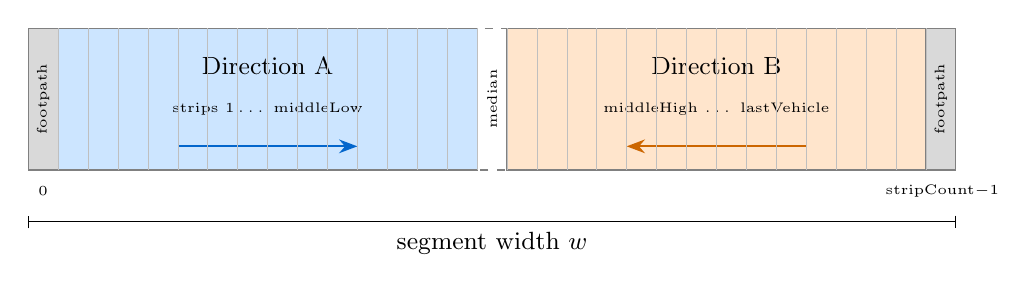
\begin{tikzpicture}[x=0.19cm, y=0.6cm]
    % footpath near
    \fill[stripFoot, draw=black!50] (0,0) rectangle (2,3);
    \node[rotate=90, font=\tiny] at (1,1.5) {footpath};
    % direction A
    \fill[stripA, draw=black!50] (2,0) rectangle (30,3);
    \node[font=\small] at (16,2.2) {Direction A};
    \node[font=\tiny] at (16,1.3) {strips $1 \dots$ middleLow};
    \draw[-{Stealth}, thick, primaryblue] (10,0.5) -- (22,0.5);
    % median
    \fill[white, draw=black!50, dashed] (30,0) rectangle (32,3);
    \node[rotate=90, font=\tiny] at (31,1.5) {median};
    % direction B
    \fill[stripB, draw=black!50] (32,0) rectangle (60,3);
    \node[font=\small] at (46,2.2) {Direction B};
    \node[font=\tiny] at (46,1.3) {middleHigh $\dots$ lastVehicle};
    \draw[-{Stealth}, thick, orange!80!black] (52,0.5) -- (40,0.5);
    % footpath far
    \fill[stripFoot, draw=black!50] (60,0) rectangle (62,3);
    \node[rotate=90, font=\tiny] at (61,1.5) {footpath};
    % strip ticks
    \foreach \x in {2,4,...,60} { \draw[black!25, very thin] (\x,0) -- (\x,3); }
    % labels
    \node[font=\tiny] at (1,-0.45) {0};
    \node[font=\tiny] at (61,-0.45) {\,stripCount$-1$};
    \draw[|-|] (0,-1.1) -- (62,-1.1) node[midway, below, font=\small] {segment width $w$};
\end{tikzpicture}
\end{center}

\begin{table}[h!]
\centering
\begin{tabularx}{\textwidth}{l l X}
\toprule
\textbf{Region} & \textbf{Strip range} & \textbf{Meaning} \\
\midrule
Footpath (near) & \code{0} & pedestrians, parked objects \\
Direction A & \code{1 \dots middleLowStripIndex} & forward travel \\
Median & (odd \code{stripCount} only) & unused divider strip \\
Direction B & \code{middleHighStripIndex \dots lastVehicleStripIndex} & reverse travel \\
Footpath (far) & \code{stripCount-1} & pedestrians, parked objects \\
\bottomrule
\end{tabularx}
\caption{Strip regions within a segment.}
\end{table}

\subsection{Worked example --- the shipped Dhaka network}

With \code{StripWidth 0.5} and \code{FootpathStripWidth 0.5}:

\begin{table}[h!]
\centering
\begin{tabular}{r r c c c}
\toprule
\textbf{Road width} & \textbf{Strips} & \textbf{Direction A} & \textbf{Direction B} & \textbf{Footpaths} \\
\midrule
24.5\,m & 49 & 1--23 & 25--47 & 0, 48 \\
27.0\,m & 54 & 1--26 & 27--52 & 0, 53 \\
32.0\,m & 64 & 1--31 & 32--62 & 0, 63 \\
\bottomrule
\end{tabular}
\caption{Strip layout of the three road widths present in the shipped network.}
\end{table}

A 27\,m road therefore offers 26 strips per direction --- enough for five buses
abreast, or thirteen motorbikes.

\subsection{Vehicle footprint}

\[
    \text{numberOfStrips} = \left\lceil
        \frac{\text{vehicleWidth}}{\text{StripWidth}} \right\rceil
\]

A vehicle at $\text{stripIndex}=k$ occupies strips
$k \dots k+\text{numberOfStrips}-1$ and registers itself in the vehicle list of
every one of them (\code{Vehicle.\_occupy\_strips}). All neighbour searches ---
leader, follower, gap checks, collision checks --- iterate those strips. Leaving
a strip is \code{Vehicle.free\_strips()}; a lateral move is
\code{Vehicle.\_change\_strip()}.

\subsection{Longitudinal position}

\code{distanceInSegment} is the position of the \textbf{tail} of the vehicle
measured from the segment start, so the head is at
$\text{distanceInSegment} + \text{length}$. A vehicle starts at $0.1$\,m and is
considered at the segment end when
\[
    \text{distanceInSegment} + \text{length} + \text{MARGIN}
    \;\geq\; \text{segmentLength}, \qquad \text{MARGIN} = 1\,\text{m}
\]
For a vehicle travelling in direction B (\code{reverseSegment = True}) the
geometry is mirrored when drawing and when comparing against pedestrian and
object positions, but \code{distanceInSegment} still counts up from that
vehicle's own entry end.

%======================================================================
\section{Architecture --- How the Simulator Works}

\subsection{Execution flow}

\begin{center}
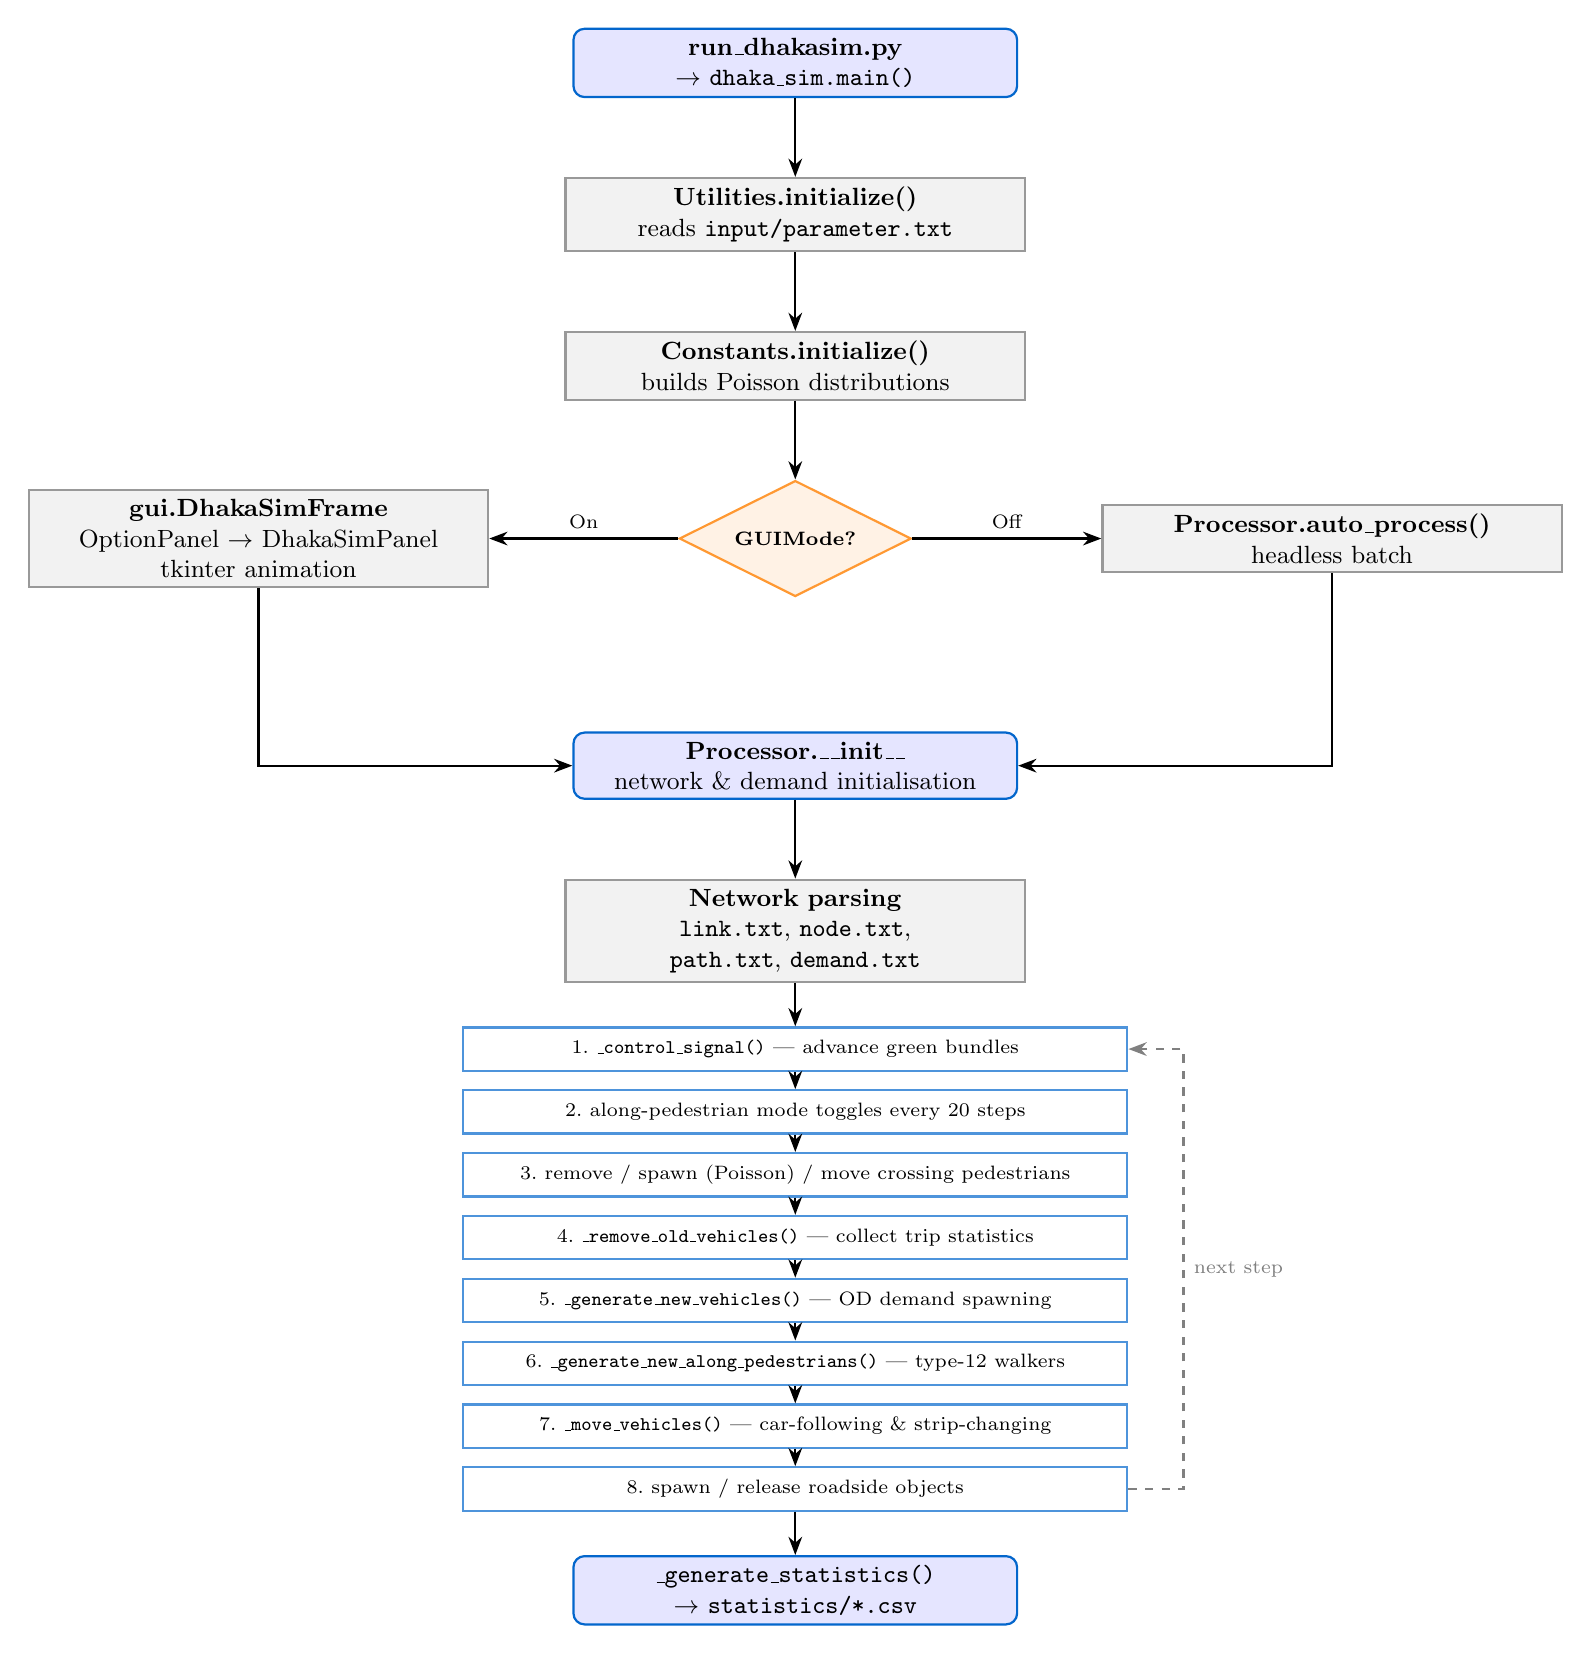
\begin{tikzpicture}[node distance=1.0cm and 1.6cm, auto, >=Stealth]
    \tikzstyle{start} = [rectangle, rounded corners, draw=primaryblue, fill=blue!10, thick, text width=5.4cm, align=center, minimum height=0.8cm, font=\small]
    \tikzstyle{process} = [rectangle, draw=gray!80, fill=gray!10, thick, text width=5.6cm, align=center, minimum height=0.8cm, font=\small]
    \tikzstyle{decision} = [diamond, draw=orange!80, fill=orange!10, thick, text width=1.9cm, align=center, aspect=2, font=\scriptsize]
    \tikzstyle{substep} = [rectangle, draw=primaryblue!70, fill=white, thick, text width=8.2cm, align=center, minimum height=0.55cm, font=\scriptsize]

    \node (main)  [start]                       {\textbf{run\_dhakasim.py} $\rightarrow$ \code{dhaka\_sim.main()}};
    \node (init)  [process, below=of main]      {\textbf{Utilities.initialize()}\\reads \code{input/parameter.txt}};
    \node (cinit) [process, below=of init]      {\textbf{Constants.initialize()}\\builds Poisson distributions};
    \node (dec)   [decision, below=of cinit]    {\textbf{GUIMode?}};
    \node (gui)   [process, left=of dec, xshift=-0.8cm]  {\textbf{gui.DhakaSimFrame}\\OptionPanel $\rightarrow$ DhakaSimPanel\\tkinter animation};
    \node (head)  [process, right=of dec, xshift=0.8cm]  {\textbf{Processor.auto\_process()}\\headless batch};
    \node (proc)  [start, below=of dec, yshift=-0.7cm]   {\textbf{Processor.\_\_init\_\_}\\network \& demand initialisation};
    \node (read)  [process, below=of proc]      {\textbf{Network parsing}\\\code{link.txt}, \code{node.txt}, \code{path.txt}, \code{demand.txt}};

    \node (s1) [substep, below=0.55cm of read] {1.\ \code{\_control\_signal()} --- advance green bundles};
    \node (s2) [substep, below=0.22cm of s1]   {2.\ along-pedestrian mode toggles every 20 steps};
    \node (s3) [substep, below=0.22cm of s2]   {3.\ remove / spawn (Poisson) / move crossing pedestrians};
    \node (s4) [substep, below=0.22cm of s3]   {4.\ \code{\_remove\_old\_vehicles()} --- collect trip statistics};
    \node (s5) [substep, below=0.22cm of s4]   {5.\ \code{\_generate\_new\_vehicles()} --- OD demand spawning};
    \node (s6) [substep, below=0.22cm of s5]   {6.\ \code{\_generate\_new\_along\_pedestrians()} --- type-12 walkers};
    \node (s7) [substep, below=0.22cm of s6]   {7.\ \code{\_move\_vehicles()} --- car-following \& strip-changing};
    \node (s8) [substep, below=0.22cm of s7]   {8.\ spawn / release roadside objects};
    \node (fin) [start, below=0.55cm of s8]    {\code{\_generate\_statistics()} $\rightarrow$ \code{statistics/*.csv}};

    \draw [->, thick] (main) -- (init);
    \draw [->, thick] (init) -- (cinit);
    \draw [->, thick] (cinit) -- (dec);
    \draw [->, thick] (dec) -- node[above, font=\scriptsize] {On} (gui);
    \draw [->, thick] (dec) -- node[above, font=\scriptsize] {Off} (head);
    \draw [->, thick] (gui) |- (proc);
    \draw [->, thick] (head) |- (proc);
    \draw [->, thick] (proc) -- (read);
    \draw [->, thick] (read) -- (s1);
    \draw [->, thick] (s1) -- (s2);
    \draw [->, thick] (s2) -- (s3);
    \draw [->, thick] (s3) -- (s4);
    \draw [->, thick] (s4) -- (s5);
    \draw [->, thick] (s5) -- (s6);
    \draw [->, thick] (s6) -- (s7);
    \draw [->, thick] (s7) -- (s8);
    \draw [->, thick] (s8) -- (fin);
    % loop-back arrow
    \draw [->, thick, dashed, gray] (s8.east) -- ++(0.7,0) |- node[right, font=\scriptsize, align=left, pos=0.25]
        {next step} (s1.east);
\end{tikzpicture}
\end{center}

\subsection{Startup sequence}

\begin{enumerate}
    \item \textbf{\code{run\_dhakasim.py}} puts the package on \code{sys.path}
          and calls \code{dhakasim.dhaka\_sim.main()}.
    \item \textbf{\code{Utilities.initialize()}} parses
          \code{input/parameter.txt} into the \code{Parameters} class
          attributes: strip geometry, pixel scaling, active behavioural models,
          and the random seed.
    \item \textbf{\code{Constants.initialize()}} builds the two Poisson
          pedestrian-arrival distributions. This is deliberately separate from
          module import, because the distribution means come from
          \code{parameter.txt} and so cannot exist until step 2 has run.
    \item \textbf{\code{Utilities.index\_trace\_file()}} indexes
          \code{trace.txt} when \code{TraceMode On}, so the GUI's trace slider
          can seek to any step.
    \item \textbf{Mode branching} on \code{Parameters.GUI\_MODE} (overridable
          with \code{--headless} / \code{--gui}):
    \begin{itemize}
        \item \textbf{GUI}: \code{DhakaSimFrame} shows \code{OptionPanel};
              pressing \emph{Start Simulation} applies the form values, creates
              \code{DhakaSimPanel}, and starts a \code{tkinter.after} timer that
              drives one step per tick.
        \item \textbf{Headless}: \code{Processor().auto\_process()} runs the loop
              to completion.
    \end{itemize}
    \item \textbf{\code{Processor.\_\_init\_\_}} reads the network, routes and
          demand, resets \code{Statistics}, creates \code{statistics/}, and
          computes the per-route generation schedule.
\end{enumerate}

\subsection{Layering}

\begin{center}
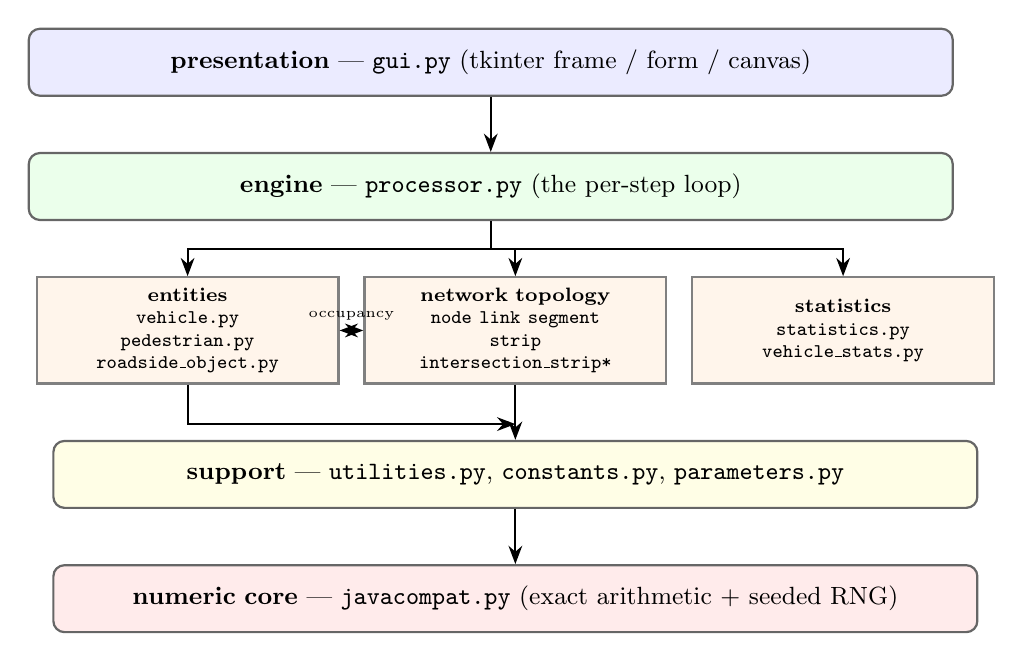
\begin{tikzpicture}[node distance=0.7cm, >=Stealth]
    \tikzstyle{layer} = [rectangle, rounded corners, draw=black!60, thick, text width=11.5cm, align=center, minimum height=0.85cm, font=\small]
    \tikzstyle{sub}   = [rectangle, draw=black!50, thick, text width=3.6cm, align=center, minimum height=1.35cm, font=\scriptsize]

    \node (pres) [layer, fill=blue!8]  {\textbf{presentation} --- \code{gui.py} (tkinter frame / form / canvas)};
    \node (eng)  [layer, fill=green!8, below=of pres] {\textbf{engine} --- \code{processor.py} (the per-step loop)};

    \node (ent)  [sub, fill=orange!8, below left=0.7cm and -0.1cm of eng.south west, anchor=north west]
        {\textbf{entities}\\\code{vehicle.py}\\\code{pedestrian.py}\\\code{roadside\_object.py}};
    \node (net)  [sub, fill=orange!8, right=0.3cm of ent]
        {\textbf{network topology}\\\code{node} \code{link} \code{segment}\\\code{strip}\\\code{intersection\_strip*}};
    \node (stat) [sub, fill=orange!8, right=0.3cm of net]
        {\textbf{statistics}\\\code{statistics.py}\\\code{vehicle\_stats.py}};

    \node (sup)  [layer, fill=yellow!10, below=0.7cm of net.south, anchor=north]
        {\textbf{support} --- \code{utilities.py}, \code{constants.py}, \code{parameters.py}};
    \node (compat)[layer, fill=red!8, below=of sup]
        {\textbf{numeric core} --- \code{javacompat.py} (exact arithmetic + seeded RNG)};

    \draw [->, thick] (pres) -- (eng);
    \draw [->, thick] (eng.south) -- ++(0,-0.35) -| (ent.north);
    \draw [->, thick] (eng.south) -- ++(0,-0.35) -| (net.north);
    \draw [->, thick] (eng.south) -- ++(0,-0.35) -| (stat.north);
    \draw [<->, thick] (ent) -- node[above, font=\tiny] {occupancy} (net);
    \draw [->, thick] (ent.south) |- ($(sup.north)+(0,0.2)$);
    \draw [->, thick] (net) -- (sup);
    \draw [->, thick] (sup) -- (compat);
\end{tikzpicture}
\end{center}

\code{javacompat.py} sits underneath everything: it supplies the arithmetic
primitives (\code{jmin}, \code{jround}, \code{jdiv}, \code{JavaRandom}, \dots)
that the whole simulator is built on. See Section~\ref{sec:compat}.

%======================================================================
\section{Repository Layout}

\begin{lstlisting}[caption=Repository layout]
DhakaSIM_python/
|-- input/                          scenario definition (read at startup)
|   |-- parameter.txt               all runtime settings
|   |-- link.txt                    links and their segments (geometry, width)
|   |-- node.txt                    intersections and boundary nodes
|   |-- path.txt                    routes (link sequences) per OD pair
|   |-- demand.txt                  vehicles/hour per OD pair
|   |-- demand_all.txt              unthinned demand from run_sim.py
|   `-- demand-low/medium/high.txt  alternative demand levels
|-- dhakasim/                       the simulator package
|-- run_dhakasim.py                 launcher
|-- run_sim.py                      route + demand generator (Floyd-Warshall)
|-- tests/test_javacompat.py        numeric regression tests
|-- README.md                       user-facing quick start
`-- DhakaSIM_Python_Codebase_Analysis.{md,tex}   this document
\end{lstlisting}

Generated at run time (git-ignored): \code{statistics/}, \code{trace.txt},
\code{debug/}.

%======================================================================
\section{Module Reference}

\subsection{Network topology layer}

\begin{tabularx}{\textwidth}{l r X}
\toprule
\textbf{Module} & \textbf{Lines} & \textbf{Purpose / Functionality} \\
\midrule
\code{node.py} & 277 & Intersections. Owns \code{IntersectionStripBundle}s (one per incoming link) carrying signal state, the list of \code{IntersectionStrip}s (turn paths through the junction), and the vehicles currently inside. Runs separating-axis collision detection between vehicles in the junction. A node with more than one link is a signalised junction. \\
\code{link.py} & 57 & Connects two nodes (\code{upNode}, \code{downNode}); an ordered list of \code{Segment}s. \\
\code{segment.py} & 293 & A straight road stretch: start/end coordinates, width, the strip array, a mid-point sensor, and per-segment counters (throughput, average speed, waiting time, accidents). Computes the strip layout of Section~\ref{sec:strips}. \\
\code{strip.py} & 528 & The spatial unit. Holds the vehicle, pedestrian and object lists occupying it, and answers every neighbour query: \code{probable\_leader}, \code{probable\_follower}, \code{probable\_object\_leader}, \code{has\_gap\_for\_adding\_vehicle}, \code{has\_gap\_for\_strip\_change} (where the lane-changing models live), \code{get\_gap\_for\_forward\_movement}, \code{has\_collision\_occurred}, \code{check\_for\_accident}. \\
\code{intersection\_strip.py} & 35 & One turn path across a junction: entry strip $\rightarrow$ exit strip, with the two pixel-space endpoints defining its centre line. \\
\code{intersection\_strip\_bundle.py} & 58 & All turn paths that \emph{enter} the junction from one link, sharing a single signal state. Signal control operates on bundles, not individual turns. \\
\code{link\_segment\_orientation.py} & 45 & Given a point and a link, decides whether the vehicle traverses the link forwards or backwards (\code{reverseLink}) and whether the segment is entered from its start or its end (\code{reverseSegment}). Everything directional keys off these two flags. \\
\bottomrule
\end{tabularx}

\subsection{Traffic entity layer}

\begin{tabularx}{\textwidth}{l r X}
\toprule
\textbf{Module} & \textbf{Lines} & \textbf{Purpose / Functionality} \\
\midrule
\code{vehicle.py} & 2{,}309 & The main entity. Physical properties from type; longitudinal control (13 car-following models); lateral control (strip changing); junction traversal including deadlock escape; fuel consumption; collision/accident bookkeeping; drawing geometry. \\
\code{pedestrian.py} & 218 & A \textbf{road-crossing} pedestrian: moves laterally across the strips one at a time (\code{move\_forward}), and shuffles longitudinally (\code{move\_length\_wise}) when blocked. Removed on reaching the far side or when stuck longer than $\text{segmentWidth}/\text{speed}$. \\
\code{roadside\_object.py} & 207 & A stationary side-friction element: standing pedestrian, parked car, parked rickshaw, parked CNG. Occupies a contiguous block of strips from the footpath inwards for a randomly drawn parking duration. \\
\bottomrule
\end{tabularx}

\medskip
Pedestrians walking \textbf{along} the road are not \code{Pedestrian} objects ---
they are \code{Vehicle}s of type 12 with a $0.4 \times 0.4$\,m footprint. This
lets them participate in car-following and strip-changing like any other road
user.

\subsection{Simulation engine layer}

\begin{tabularx}{\textwidth}{l r X}
\toprule
\textbf{Module} & \textbf{Lines} & \textbf{Purpose / Functionality} \\
\midrule
\code{processor.py} & 1{,}367 & The engine. Network/route/demand parsing, per-step orchestration, vehicle and pedestrian and object generation, signal control, junction entry/exit, flow measurement, final statistics output. \\
\code{parameters.py} & 98 & Every runtime setting as class attributes (Java \code{static} fields), plus the three model enumerations. \\
\code{constants.py} & 130 & Fixed physical constants, colours, and the empirical Gaussian-mixture blockage distributions for the four roadside object types, derived from Dhaka field survey data. \\
\code{statistics.py} & 60 & Global accumulators, reset per run. \\
\code{vehicle\_stats.py} & 37 & Per-vehicle speed and trajectory time series (written out only when \code{Processor.write\_speed()} is enabled). \\
\code{dhaka\_sim.py} & 37 & Entry point: initialise, then branch on GUI mode. \\
\bottomrule
\end{tabularx}

\subsection{Support layer}

\begin{tabularx}{\textwidth}{l r X}
\toprule
\textbf{Module} & \textbf{Lines} & \textbf{Purpose / Functionality} \\
\midrule
\code{utilities.py} & 658 & Parameter file parsing; 2-D geometry helpers (\code{return\_x3} \dots \code{return\_y6} compute the perpendicular offsets used for road and vehicle corners); the error function and Gaussian CDF; per-type vehicle dimensions and performance; blockage sampling from the Gaussian mixtures; the strip-weight function used by the strip-based car-following model. \\
\code{javacompat.py} & 640 & Exact numeric semantics and the seeded RNG. See Section~\ref{sec:compat}. \\
\code{demand.py} & 40 & An OD pair with its flow rate and the routes serving it. \\
\code{path.py} & 33 & A route: source node, destination node, ordered link ids. \\
\code{point2d.py}, \code{signal.py}, \code{normal\_distribution.py} & 14/16/39 & A mutable 2-D point; the \code{RED}/\code{GREEN}/\code{YELLOW} enum; a single Gaussian component of a mixture. \\
\bottomrule
\end{tabularx}

\subsection{Presentation \& tooling}

\begin{tabularx}{\textwidth}{l r X}
\toprule
\textbf{Module} & \textbf{Lines} & \textbf{Purpose / Functionality} \\
\midrule
\code{gui.py} & 549 & \code{DhakaSimFrame} (window), \code{OptionPanel} (parameter form), \code{DhakaSimPanel} (animated canvas), and \code{CanvasGraphics} --- an adapter applying the pan/zoom transform and drawing onto a \code{tkinter.Canvas}. Also writes and replays \code{trace.txt}. \\
\code{run\_sim.py} & 281 & Floyd--Warshall route generator: builds node adjacency from \code{link.txt}/\code{node.txt}, computes shortest paths between all boundary node pairs, writes \code{path.txt} + \code{demand.txt}. \\
\code{tests/test\_javacompat.py} & 131 & Pins the numeric layer to reference values. \\
\bottomrule
\end{tabularx}

%======================================================================
\section{The Simulation Loop, Step by Step}
\label{sec:loop}

\code{Processor.\_run\_at\_each\_time\_step()} executes exactly this order once
per simulated second. \textbf{The order matters} --- several stages depend on
state written by an earlier one.

\begin{tabularx}{\textwidth}{c l X}
\toprule
\textbf{\#} & \textbf{Call} & \textbf{What happens} \\
\midrule
1 & \code{\_control\_signal()} & Only when $\text{step} \bmod \text{SignalChangeDuration} = 0$. Advances the green bundle at every signalised node. \\
2 & \emph{(toggle)} & If along-pedestrian mode was on at startup, \code{along\_pedestrian\_mode} flips every 20 steps, producing alternating 20-second bursts of footpath pedestrian traffic. \\
3 & \code{\_remove\_old\_pedestrians()} \code{\_generate\_new\_pedestrians()} \code{\_move\_pedestrians()} & Only when \code{AcrossPedestrianMode On}. Drop finished pedestrians, Poisson-spawn new ones per link, then move each one laterally (or longitudinally if blocked). \\
4 & \code{\_remove\_old\_vehicles()} & Vehicles flagged \code{toRemove} free their strips, contribute to trip statistics, and leave the list. \\
5 & \code{\_generate\_new\_vehicles()} & For every route whose next generation time has arrived, spawn vehicle(s) and schedule the next arrival. \\
6 & \code{\_generate\_new\_along\_pedestrians()} & Only while \code{along\_pedestrian\_mode} is currently true. Poisson-spawns type-12 pedestrian ``vehicles''. \\
7 & \code{\_move\_vehicles()} & The main movement pass --- see below. \\
8 & \code{\_generate\_new\_objects()} \code{\_remove\_old\_objects()} & Only when \code{ObjectMode On}. Spawn parked vehicles / standing pedestrians, then release those whose parking time expired. \\
\bottomrule
\end{tabularx}

\subsection{Inside \code{\_move\_vehicles()}}

For each vehicle, in list order (which is creation order):

\begin{lstlisting}[language=Python, caption=Movement dispatch (pseudocode)]
if PenaltyWait and vehicle already collided:
    if penalty time elapsed: remove from simulation
    skip this vehicle
if vehicle is inside a junction:
    free its strips (it is not on a segment)
    if at junction exit:  move_vehicle_at_intersection_end()   # enter next link
    else:                 move_vehicle_in_intersection()
                          then re-check for arrival at the exit
else:
    look up the signal ahead and store it on the vehicle
    if at segment end:    move_vehicle_at_segment_end()        # next segment, or junction
    else:                 move_vehicle_at_segment_middle()     # ordinary driving
                          then re-check for arrival at the end
increment fuel consumption; record speed and position
\end{lstlisting}

Then two separate passes over all vehicles:
\begin{enumerate}
    \item \code{accident\_log\_all\_vehicle\_at\_last()} --- appends a row to
          \code{statistics/accident\_log.csv} for any vehicle that has collided
          or struck a pedestrian.
    \item \code{accident\_check\_all\_vehicles\_at\_last()} --- intended to apply
          the collision penalty. See quirk~\ref{quirk:accidents}: in practice it
          never fires, because the check in pass 1 consumes the pedestrian.
\end{enumerate}

Finally, every 60 steps the minute's \code{flowCount} is written into
\code{Statistics.flow} and reset.

\subsection{Ordinary driving --- \code{Vehicle.move\_vehicle\_in\_segment()}}

For everything except type-12 pedestrians:

\begin{lstlisting}[language=Python]
if is_object_in_proximity() or not move_forward_in_segment() or is_slower_vehicle_in_proximity():
    try_lane_change(priority_towards_middle=True)
\end{lstlisting}

Read it as: \emph{if a parked object is ahead, or I could not move forward at
all, or my leader is slower than I want to go --- try to change strips.} The
three conditions are evaluated left to right and
\code{move\_forward\_in\_segment()} has the side effect of actually moving, so
the ordering is load-bearing. A lane change is attempted towards the road centre
first, then towards the kerb --- except that a vehicle will not move towards the
kerb when a parked object is there.

Type-12 pedestrians take a different branch: with probability
\code{PedestrianRandomLaneChangePercentage}/101 they attempt a random lateral
move (biased left with probability \code{PedestrianLeftBiasPercentage}/101),
otherwise they walk forward and only swerve if blocked.

\subsection{Moving forward --- \code{Vehicle.\_move\_forward\_in\_segment()}}

\begin{enumerate}
    \item \code{\_control\_speed\_in\_segment()} picks the new speed from the
          active car-following model, clamps it to \code{currentMaxSpeed}, and
          --- if \code{BrakeHard On} --- further clamps it to the smallest
          actually-available gap across all occupied strips.
    \item If the speed is usable, the position advances by \textbf{Butcher's
          fifth-order quadrature} rather than $x + v\Delta t$:
    \begin{align*}
        \Delta v &= v_{\text{new}} - v_{\text{old}} \\
        k_1 &= v_{\text{old}}, \quad
        k_3 = v_{\text{old}} + 0.25\Delta v, \quad
        k_4 = v_{\text{old}} + 0.50\Delta v \\
        k_5 &= v_{\text{old}} + 0.75\Delta v, \quad
        k_6 = v_{\text{new}} \\
        x_{\text{new}} &= x + \tfrac{1}{90}\left(7k_1 + 32k_3 + 12k_4 + 32k_5 + 7k_6\right)\Delta t
    \end{align*}
    \item The position is capped so the vehicle never overruns the segment end,
          and the mid-segment sensor flag is set the first time it is passed.
    \item If the speed was zero, \code{waitingTime} and
          \code{waitingTimeInSegment} both increment --- this is what the
          waiting-time statistics measure.
\end{enumerate}

%======================================================================
\section{Vehicle Generation \& Demand}
\label{sec:demand}

\subsection{From \code{demand.txt} to a spawn schedule}

\code{Processor.\_read\_demand()} reads \code{source dest vehiclesPerHour} and
stores \textbf{\code{vehiclesPerHour + 30}} --- a hard-coded offset applied to
every route, so a file value of 100 becomes an effective 130\,veh/h.

For each route:
\begin{align*}
    \text{demandRatio} &= 3600 / \text{demand} \\
    \text{vehiclesToGenerate} &= 1 \quad\text{if demandRatio} > 1, \quad
        \text{else } \text{round}(1/\text{demandRatio}) \\
    \text{nextGenerationTime} &= 1
\end{align*}
\code{vehiclesToGenerate} only exceeds 1 for demands above 3600\,veh/h, so with
normal inputs one spawn attempt is made per arrival event.

\subsection{Arrival process}

\code{\_generate\_new\_vehicles()} fires when \code{nextGenerationTime} equals
the current step, then repeats until the next arrival falls in a later step:

\begin{center}
\begin{tabularx}{\textwidth}{l X}
\toprule
\textbf{\code{VehicleGenerationRate}} & \textbf{Headway} \\
\midrule
\code{0} --- CONSTANT & $X = 3600/\text{demand}$ (deterministic) \\
\code{1} --- POISSON & $X = (3600/\text{demand})\cdot(-\ln U)$, $U \sim \text{Uniform}(0,1)$ --- exponential inter-arrival times, i.e.\ a Poisson process \\
\bottomrule
\end{tabularx}
\end{center}

\subsection{Placing the vehicle}

\code{\_create\_a\_vehicle()}:
\begin{enumerate}
    \item Pick a route uniformly among those serving the OD pair.
    \item Pick a vehicle type from the mix (below).
    \item Resolve the entry segment and its orientation, then the legal strip
          window for the travel direction (\code{1 \dots middleLow} or
          \code{middleHigh \dots lastVehicle}).
    \item Pick a random start strip in that window, then scan \textbf{upwards}
          for a strip run wide enough and clear enough for the vehicle
          (\code{has\_gap\_for\_adding\_vehicle}, which requires the first
          $\text{THRESHOLD\_DISTANCE} + 0.08 + \text{length}$ metres to be free
          of vehicles, objects and pedestrians). If nothing is found, scan
          \textbf{downwards}.
    \item If no gap exists anywhere, the vehicle is simply \textbf{not created}
          --- demand is lost rather than queued. This is how the model saturates.
\end{enumerate}

\subsection{Vehicle type mix}
\label{sec:mix}

\code{\_distributed\_vehicle\_type()} draws
$\text{ratio} = \text{randomInt}(0..100)$ and, after the percentage split is
forced to slow~25 / medium~25 / fast~50, resolves to:

\begin{table}[h!]
\centering
\begin{tabular}{l r l l}
\toprule
\textbf{Band} & \textbf{Prob.} & \textbf{Sub-draw} & \textbf{Type} \\
\midrule
Slow ($\text{ratio} < 25$)   & $\approx$24.8\,\% & $<9$      & 0 bicycle \\
                             &                   & $9..97$   & 1 rickshaw \\
                             &                   & $\geq 98$ & 2 van / pushcart \\
\midrule
Medium ($25 \leq \text{ratio} < 50$) & $\approx$24.8\,\% & $<83$     & 7 CNG \\
                             &                   & $83..97$  & 8--9 bus \\
                             &                   & $\geq 98$ & 10--11 truck \\
\midrule
Fast ($\text{ratio} \geq 50$)& $\approx$50.5\,\% & $<88$     & 3 motorbike \\
                             &                   & $\geq 88$ & 4--6 car \\
\bottomrule
\end{tabular}
\caption{Vehicle type composition actually generated.}
\end{table}

The result is a heavily rickshaw- and motorbike-dominated stream, which is the
point: it reproduces observed Dhaka composition rather than a Western vehicle
mix. Three alternative mixes are present but unused ---
\code{\_distributed\_vehicle\_type\_miami()},
\code{\_distributed\_vehicle\_type\_bd\_new()},
\code{\_random\_vehicle\_type()} --- and can be swapped in at
\code{\_pedestrian\_vehicle\_distribution\_type()}.

%======================================================================
\section{Vehicle Types}

Defined in \code{utilities.py} (\code{\_CAR\_WIDTHS}, \code{\_CAR\_LENGTHS},
\code{\_CAR\_SPEEDS}, \code{\_CAR\_ACCELERATIONS}). Maximum braking is
$-6$\,m/s\textsuperscript{2} for every type.

\begin{table}[h!]
\centering
\begin{tabular}{c l r r c r r r}
\toprule
\textbf{Type} & \textbf{Vehicle} & \textbf{Width} & \textbf{Length} & \textbf{Strips} & \multicolumn{2}{c}{\textbf{Max speed}} & \textbf{Accel} \\
 & & (m) & (m) & @0.5\,m & (km/h) & (m/s) & (m/s\textsuperscript{2}) \\
\midrule
0  & bicycle                 & 0.55 & 1.90  & 2 & 15  & 4.1666  & 0.42 \\
1  & rickshaw                & 1.20 & 2.40  & 3 & 8   & 2.2222  & 0.25 \\
2  & van / pushcart          & 1.22 & 2.50  & 3 & 7   & 1.9444  & 0.20 \\
3  & motorbike               & 0.60 & 1.80  & 2 & 100 & 27.7777 & 2.80 \\
4  & car                     & 1.70 & 5.00  & 4 & 100 & 27.7777 & 3.00 \\
5  & car                     & 1.76 & 4.55  & 4 & 60  & 16.6666 & 2.80 \\
6  & car                     & 1.78 & 4.30  & 4 & 110 & 30.5555 & 3.34 \\
7  & CNG (auto-rickshaw)     & 1.40 & 2.65  & 3 & 40  & 11.1111 & 1.11 \\
8  & bus                     & 2.40 & 10.30 & 5 & 30  & 8.3333  & 0.84 \\
9  & bus                     & 2.30 & 9.50  & 5 & 40  & 11.1111 & 1.12 \\
10 & truck                   & 2.44 & 7.20  & 5 & 35  & 9.7222  & 0.96 \\
11 & truck                   & 2.46 & 7.50  & 5 & 45  & 12.5000 & 1.24 \\
12 & pedestrian (along road) & 0.40 & 0.40  & 1 & 5.1 & 1.4166  & 0.10 \\
\bottomrule
\end{tabular}
\caption{The 13 vehicle types. Column order in every per-type CSV.}
\end{table}

Two details:
\begin{itemize}
    \item The effective ceiling is
          $\min(\text{MaximumSpeed}, \text{typeMaxSpeed})$, so the network speed
          limit can bind before the vehicle's own capability does.
    \item Type 12 gets \textbf{per-individual variation}: its max speed and
          acceleration are each perturbed by a Gaussian with
          $\sigma = \text{mean}/5$, so a crowd of walkers has a realistic speed
          spread.
\end{itemize}

%======================================================================
\section{Car-Following Models}
\label{sec:cf}

Selected by \code{CF\_model} in \code{input/parameter.txt}. All are implemented
in \code{vehicle.py}; each returns a new speed, from which acceleration is
back-computed as $(v_{\text{new}} - v_{\text{old}})/\Delta t$.

\begin{table}[h!]
\centering
\begin{tabular}{c l l}
\toprule
\textbf{\code{CF\_model}} & \textbf{Model} & \textbf{Method} \\
\midrule
0  & \textbf{HYBRID} (default)              & \code{\_get\_new\_speed\_gipps\_model} \\
1  & NAIVE                                  & inline --- accelerate maximally, ignore everything \\
2  & GIPPS                                  & \code{\_get\_new\_speed\_gipps\_model} \\
3  & KRAUSS                                 & \code{\_get\_new\_speed\_krauss\_model} \\
4  & GFM (generalised force)                & \code{\_get\_new\_speed\_gfm\_model} \\
5  & IDM (intelligent driver)               & \code{\_get\_new\_speed\_idm\_model} \\
6  & RVF (reduced visual field)             & \code{\_get\_new\_speed\_rvf\_model} \\
7  & VFIAC                                  & \code{\_get\_new\_speed\_vfiac\_model} \\
8  & OVCM (optimal velocity, memory)        & \code{\_get\_new\_speed\_ovcm\_model} \\
9  & KFTM                                   & \code{\_get\_new\_speed\_kftm\_model} \\
10 & HDM (human driver, multi-leader)       & \code{\_get\_new\_speed\_hdm\_model} \\
11 & SBM (stochastic behavioural)           & \code{\_get\_new\_speed\_sbm\_model} \\
12 & \textbf{MY\_MODEL} (strip-based)       & \code{\_get\_new\_speed\_my\_model} \\
\bottomrule
\end{tabular}
\caption{Available car-following models.}
\end{table}

\subsection{Gap definition}

Every model works from the same gap, in \code{Vehicle.get\_gap()}:
\[
    \Delta x = x_{\text{leader}} - \text{THRESHOLD\_DISTANCE}
             - \left(x_{\text{follower}} + \text{length}_{\text{follower}}\right)
\]
i.e.\ bumper-to-bumper clearance minus a 0.5\,m standstill buffer. The gap can go
\textbf{negative}, which is how overlaps (collisions) become detectable.

When \code{ErrorMode On}, \code{get\_dx()} instead returns a \emph{perceived} gap
corrupted by sensor error --- radar error for the immediate leader, GPS position
error for further leaders --- controlled by \code{FTMethod},
\code{NoOfReadings} and \code{MFactor}. This supports connected/automated-vehicle
experiments.

\subsection{Gipps / hybrid (the default)}

Free-flow branch --- how fast the driver \emph{wants} to go:
\[
    v_a = v_n + 2.5\,a_n T \left(1 - \frac{v_n}{V_n}\right)
          \sqrt{0.025 + \frac{v_n}{V_n}}
\]
Car-following branch --- the fastest speed from which the driver can still stop
safely behind the leader:
\[
    v_b = d T + \sqrt{d^2T^2 - d\left(2\Delta x - v_n T
          - \frac{v_{n-1}^2}{\hat d}\right)}
\]
where $d$ is the follower's maximum braking ($-6$\,m/s\textsuperscript{2}), $T$
the reaction time (= 1\,s = one time step), and
$\hat d = (d_{\text{leader}} + d_{\text{follower}})/2$ the follower's estimate of
the leader's deceleration. The new speed is
$\text{precision2}\left(\max(0, \min(v_a, v_b))\right)$.

\begin{quote}
\textbf{Important:} the square root argument goes negative whenever the leader is
too close to stop behind, making $v_b$ \textbf{NaN}. Java's \code{Math.min} and
\code{Math.max} propagate NaN, so $\max(0, \min(v_a, \text{NaN}))$ is NaN, which
\code{precision2} then truncates to \textbf{0} --- an emergency stop. This is a
load-bearing behaviour, not an accident; see Section~\ref{sec:compat}.
\end{quote}

The difference between GIPPS and HYBRID is only meaningful together with
\code{BrakeHard}, which adds a hard gap-based clamp on top of the model speed.

\subsection{MY\_MODEL --- the strip-aware model}

This is the model designed for non-lane traffic, and the only one that uses the
strip structure rather than treating the road as a single lane.

\begin{enumerate}
    \item \textbf{Free speed}: $v_a = \min(\text{currentMaxSpeed}, v + a\Delta t)$.
    \item \textbf{Local density}: count distinct vehicles and pedestrians within
          the vehicle's own strips widened by $\pm\text{numberOfStrips}$, over
          the longitudinal window $[x, x + 2\,\text{length}]$, divided by 9.
    \item \textbf{Adaptive attention}: if
          $\text{density}/10 < \text{DensityPercentage}/100$ the driver ignores
          adjacent strips ($\text{sideStrips}=0$); otherwise it considers
          $\text{SideStripsToConsider}=1$ strip on each side. In free flow you
          watch only your own path; in congestion you watch your neighbours.
    \item \textbf{Congested speed} over all leaders in the attention window:
    \begin{itemize}
        \item \code{ConsiderMinimum On} $\rightarrow$ the \textbf{minimum} Gipps
              braking speed over all leaders (conservative);
        \item \code{ConsiderMinimum Off} $\rightarrow$ a \textbf{weighted
              average}, where each leader's weight is its lateral overlap with
              the follower $\times$ a normalised centrality term $\times$ a type
              weight (\code{PedestrianWeight} for pedestrians, 1 otherwise),
              capped by the closest leader's speed.
    \end{itemize}
    The weight function is \code{Utilities.get\_weight()}: a leader that only
    clips the edge of your path restrains you less than one squarely in front.
\end{enumerate}

\subsection{The remaining models}

Each is a faithful implementation of its published form, retained for the
comparative studies the simulator was built for:

\begin{itemize}
    \item \textbf{KRAUSS} --- safe-velocity formulation with a $\tau = 0.3$\,s
          reaction time.
    \item \textbf{GFM} --- generalised force model; separate attraction and
          repulsion ranges ($R_a = 15$\,m, $R_d = 80$\,m).
    \item \textbf{IDM} --- desired dynamic gap
          $s^{*} = s_0 + \max\!\left(0, vT + \frac{v\Delta v}{2\sqrt{ab}}\right)$
          with $a=3$, $b=4$, $T=1.5$\,s, acceleration exponent 4.
    \item \textbf{RVF / VFIAC} --- optimal-velocity variants that average the
          leader's speed over a 4-step memory window (\code{TIME\_WINDOW}).
    \item \textbf{OVCM} --- optimal-velocity with a 3-step gap memory
          (\code{GAP\_WINDOW}).
    \item \textbf{KFTM} --- combines an IDM-like and a Gipps-like speed and takes
          the minimum, evaluated over up to three leaders within 300\,m; tuned by
          \code{ALPHA}, \code{BETA}, \code{ETA}.
    \item \textbf{HDM} --- human driver model with explicit multi-leader
          interaction over four leaders.
    \item \textbf{SBM} --- stochastic behavioural model with Gaussian noise on
          the desired spacing.
\end{itemize}

When no leader exists, the vehicle follows a \textbf{dummy leader}: a stopped
zero-length vehicle at the link end if the vehicle is in the last segment
(speed 0 on red, 5\,m/s on green), or a vehicle at $10^8$\,m travelling at the
speed limit otherwise. This is how signals brake traffic without any
special-casing in the car-following code.

%======================================================================
\section{Lane-Changing (Strip-Changing) Models}
\label{sec:dlc}

Selected by \code{DLC\_model}. The decision is made in
\code{Strip.has\_gap\_for\_strip\_change()}, called for the target strip.

A move is only considered if the target strip is geometrically free: no vehicle
whose extent ($\pm$ threshold) overlaps the mover's, and no pedestrian inside its
footprint. Beyond that:

\begin{tabularx}{\textwidth}{c l X}
\toprule
\textbf{\code{DLC\_model}} & \textbf{Model} & \textbf{Rule} \\
\midrule
0 & \textbf{NAIVE} (default) & Geometric clearance is sufficient --- change immediately. \\
1 & GHR & Feasible if the General-Motors/GHR acceleration with respect to the new leader (and of the new follower with respect to you) stays above maximum braking. \\
2 & GIPPS & Feasible if the required deceleration for you \emph{and} for the prospective follower stays above maximum braking. \\
3 & MOBIL & Accept if the new follower's acceleration stays above $b_{\text{safe}} = -4$\,m/s\textsuperscript{2} \textbf{and} the politeness-weighted total acceleration gain exceeds $a_{\text{th}} = 0.1$\,m/s\textsuperscript{2}. \\
\bottomrule
\end{tabularx}

\medskip
For GHR and GIPPS an additional \textbf{gap-acceptance probability} is applied:
\[
    P = 1 - e^{-\lambda\left(t_{\text{gap}} - t_{\text{safe}}\right)},
    \qquad \lambda = 0.78
\]
evaluated for both the lead and lag gaps and multiplied together; the change
happens only if a uniform draw falls below $P$. This makes lane changing
stochastic rather than deterministic.

The manoeuvre itself (\code{\_move\_to\_higher\_index\_lane} /
\code{\_move\_to\_lower\_index\_lane}) walks one strip at a time towards the
limit for the travel direction, and rolls back to the original strip if it cannot
find a position from which it can also move forward.

Type-12 pedestrians always use NAIVE regardless of \code{DLC\_model}
(\code{Utilities.get\_dlc\_model}).

%======================================================================
\section{Side Friction: Pedestrians \& Roadside Objects}
\label{sec:friction}

This is what distinguishes DhakaSim from lane-based simulators, and the
distributions below come from field surveys in Dhaka.

\subsection{Road-crossing pedestrians (\code{AcrossPedestrianMode})}

\begin{itemize}
    \item \textbf{Arrival}: per link, per step, a Poisson draw with mean
          $\text{AcrossPedestrianPerHour}/3600$ (default
          $400/3600 \approx 0.111$ per link-second).
    \item \textbf{Longitudinal position}: a three-zone mixture over the crossable
          range $[9\,\text{m}, \text{length}-9\,\text{m}]$. The range is split
          into its \textbf{first 20\,\%, middle 60\,\% and last 20\,\%}, drawn
          with probabilities \textbf{0.4 / 0.2 / 0.4} --- so 80\,\% of crossings
          happen in the 40\,\% of the block nearest the two junctions, which is
          what is observed on the ground.
    \item \textbf{Speed}: 0.05 or 0.15\,m/s (chosen uniformly) --- deliberately
          slow, because this value is the lateral progress per second across the
          strips.
    \item \textbf{Side}: the near or far footpath, uniformly.
    \item \textbf{Movement}: \code{move\_forward()} advances laterally into the
          next strip if that strip has a gap; if blocked,
          \code{move\_length\_wise()} shuffles along the road instead. A
          pedestrian stuck longer than $\text{segmentWidth}/\text{speed}$ is
          removed.
    \item \textbf{Effect on traffic}: a pedestrian inside a vehicle's braking
          envelope forces \code{get\_gap\_for\_forward\_movement()} to return 0
          --- a full stop --- and a pedestrian inside a vehicle's footprint
          registers an accident.
\end{itemize}

\subsection{Along-road pedestrians (\code{AlongPedestrianMode})}

Spawned as type-12 vehicles with a Poisson mean of
$\text{AlongPedestrianPerHour}/3600$ per route per step. Their initial strip
comes from the \emph{walking pedestrian} blockage distribution, so they cluster
near the kerb but stray into the carriageway realistically. Because they are
vehicles, they follow, overtake and get overtaken like everything else, and they
are weighted by \code{PedestrianWeight} when other road users decide how much to
respect them.

Note the 20-step on/off toggle described in Section~\ref{sec:loop}: footpath
pedestrian traffic arrives in bursts, not steadily.

\subsection{Roadside objects (\code{ObjectMode})}

Four types, each with an empirically fitted \textbf{mixture of Gaussians} for how
far into the carriageway it protrudes (\code{constants.py}):

\begin{table}[h!]
\centering
\begin{tabular}{c l r c c r}
\toprule
\textbf{Type} & \textbf{Object} & \textbf{L $\times$ W (m)} & \textbf{Blockage (m)} & \textbf{Components} & \textbf{Target} \\
\midrule
1 & standing pedestrian & $0.7 \times 0.7$ & 0.21--6.00 & 5 & 60 \\
2 & parked car          & $4.5 \times 1.7$ & 0.70--6.00 & 6 & 76 \\
3 & parked rickshaw     & $3.0 \times 1.0$ & 0.56--6.00 & 5 & 60 \\
4 & parked CNG          & $2.6 \times 1.3$ & 0.95--4.67 & 4 & 18 \\
5 & \emph{walking} pedestrian & --- & 0.50--7.75 & 2 & (type-12 placement) \\
\bottomrule
\end{tabular}
\caption{Roadside object types and their empirical blockage distributions.}
\end{table}

Target counts are
$\lceil \text{rate} \times \text{TOTAL\_NETWORK\_ROAD\_LENGTH} \rceil$ with
$\text{TOTAL\_NETWORK\_ROAD\_LENGTH} = 3.83$\,km.

\begin{itemize}
    \item \textbf{Spawn probability} per link per step is
          $\text{factor} \times k \times
          \left(1 - \Phi(\text{currentCount}; \text{targetCount}, 10)\right)$
          with $\text{factor}=0.1$ and $k = 3, 1, 4, 7$ for the four types. As
          the population approaches its target the Gaussian CDF drives the spawn
          rate towards zero, so counts self-regulate around the surveyed density
          instead of growing without bound.
    \item \textbf{Placement}: a random segment, a random longitudinal position in
          $[9, \text{length}-9]$, a random side, and a blockage depth drawn from
          the mixture. The object occupies every strip from the footpath up to
          its blockage depth --- and is rejected outright if any of them lacks a
          0.5\,m clear gap.
    \item \textbf{Parking duration}, drawn uniformly: standing pedestrian
          10--60\,s; parked car 100--500\,s; parked rickshaw 30--150\,s; parked
          CNG 60--300\,s. When it expires the object frees its strips and
          disappears.
    \item \textbf{Effect on traffic}: \code{is\_object\_in\_proximity()} is the
          \emph{first} condition in the movement decision, so an approaching
          object triggers a strip change before any car-following consideration
          --- and a vehicle will never change strips \emph{towards} an object.
\end{itemize}

%======================================================================
\section{Intersections \& Signals}
\label{sec:signals}

\subsection{Turn paths are created lazily}

There is no pre-computed turn table. The first time a vehicle wants to go from
(link A, strip $i$) to (link B, strip $j$),
\code{Processor.\_create\_intersection\_strip()} computes the straight-line path
across the junction between the two strip centres in pixel space and registers it
as an \code{IntersectionStrip} on the node. Subsequent vehicles reuse it. The
exit strip is derived by \code{Vehicle.get\_new\_strip\_index()}, which maps the
strip proportionally between roads of different width --- a vehicle in the third
of twenty strips arrives in roughly the third of however many strips the next
road has.

\subsection{Signals}

Turn paths entering the junction from the same link share an
\code{IntersectionStripBundle}, and the bundle carries the signal. Exactly one
bundle is green at a time; \code{constant\_signal\_change()} advances to the next
bundle once
$\text{simulationTime} - \text{timePassed} \geq \text{SignalChangeDuration}$.

\begin{quote}
With the shipped \code{SignalChangeDuration 1}, the green phase advances
\textbf{every simulated second}. That is effectively a round-robin gate rather
than a realistic signal plan --- raise it (e.g.\ 30--60) for signal-timing
studies.
\end{quote}

\code{adaptive\_signal\_change()} --- which extends green time based on the queue
pressure on the approach --- is implemented but \textbf{not called};
\code{\_control\_signal()} calls \code{constant\_signal\_change()}. Swapping the
call is a one-line change.

\subsection{Entering, traversing and leaving}

\begin{itemize}
    \item \textbf{Entering}: at the segment end, if a free strip exists in the
          entering segment and the bundle is green, the vehicle joins the node's
          vehicle list, \code{isInIntersection} becomes true, and it releases its
          segment strips. If the signal is red, or the entry is blocked, or it
          would overlap a vehicle already in the junction, its speed is set to 0.
    \item \textbf{Traversing}: inside the junction there are no strips. Collision
          avoidance uses \textbf{separating-axis testing} on the four rotated
          corner points of each vehicle (\code{Node.\_is\_colliding}).
          \code{\_control\_speed\_in\_intersection()} tries successively larger
          speeds and keeps the largest that does not overlap.
    \item \textbf{Deadlock escape}: a vehicle stuck for more than 40 steps sets
          \code{noForceMove = False}, which lets it add
          $1.5 \times \text{length}$ to its speed and jump through the blockage.
          Before that, \code{\_try\_changing\_direction\_in\_intersection()}
          attempts every alternative exit strip.
    \item \textbf{Leaving}: \code{\_move\_vehicle\_at\_intersection\_end()} finds
          a free strip in the next link, updates the route index, and resumes
          normal segment driving.
\end{itemize}

%======================================================================
\section{The Input File System --- Scenario Specification}
\label{sec:input}

Every scenario is defined purely by plain-text files in \code{input/}. No code
changes are required to model a new location.

\subsection{\code{node.txt} --- intersections and boundaries}

\begin{lstlisting}[caption=Sample node.txt]
21
0 0 0 16 18 17 14
1 317 26 4
2 436 20 19
3 675 14 20
12 0 0 15 14 13 12
\end{lstlisting}

\textbf{Format}: first line = node count; then
\code{nodeId  x  y  linkId1  linkId2  \dots}
\begin{itemize}
    \item \textbf{Boundary nodes} (exactly 1 link) are the entry/exit points of
          the network. \code{run\_sim.py} generates demand between every ordered
          pair of these.
    \item \textbf{Interior nodes} ($>1$ link) become signalised junctions. They
          conventionally carry $x=0, y=0$, because their true position is implied
          by the geometry of the links meeting there; only non-zero coordinates
          contribute to the view-centring calculation.
\end{itemize}

\subsection{\code{link.txt} --- road geometry}

\begin{lstlisting}[caption=Sample link.txt]
23
0 8 16 1
0 618 730 591 567 27
1 11 18 1
0 67 403 161 409 32
2 10 18 2
0 110 735 134 656 32
1 137 647 175 440 27
\end{lstlisting}

\textbf{Link header}: \code{linkId  upNodeId  downNodeId  segmentCount} \\
\textbf{Segment line}: \code{segmentId  startX  startY  endX  endY  width}

All values are metres. A link is a chain of straight segments, which is how
curved roads are approximated. The \textbf{width drives strip capacity} via the
formula in Section~\ref{sec:strips} --- it is the single most important number
for capacity.

\subsection{\code{path.txt} --- routes (generated)}

\begin{lstlisting}[caption=Sample path.txt]
110
1 2 4 5 9 19
1 3 4 5 9 20
\end{lstlisting}

\textbf{Format}: \code{srcNodeId  dstNodeId  linkId1  linkId2  \dots}

\subsection{\code{demand.txt} --- traffic volume matrix}

\begin{lstlisting}[caption=Sample demand.txt]
110
1 2 100
1 3 100
\end{lstlisting}

\textbf{Format}: \code{srcNodeId  dstNodeId  vehiclesPerHour}

Remember the \textbf{+30 offset} applied at load time
(Section~\ref{sec:demand}). \code{demand.txt} and \code{path.txt} must be
consistent: every demand row needs at least one matching route, or that demand is
silently unusable.

\subsection{\code{parameter.txt} --- runtime configuration}

One \code{Name Value} pair per line; unknown names are ignored, so you can leave
comments. See Section~\ref{sec:params}.

\subsection{Regenerating routes and demand}

\code{run\_sim.py} builds the node adjacency matrix from the link/node files,
runs \textbf{Floyd--Warshall} to obtain all-pairs shortest paths, emits one route
and one demand row per ordered boundary-node pair, then thins the demand
according to \code{DemandType}:

\begin{center}
\begin{tabular}{l l l}
\toprule
\textbf{\code{DemandType}} & \textbf{Accepted routes} & \textbf{Per-route rate} \\
\midrule
0 low    & $\approx 1/3$ of boundary nodes & \code{LowRate / acceptableNodes} \\
1 medium & $\approx 2/3$                   & \code{MediumRate / acceptableNodes} \\
2 high   & all                             & \code{HighRate / acceptableNodes} \\
\bottomrule
\end{tabular}
\end{center}

The unthinned file is preserved as \code{input/demand\_all.txt}.

\begin{lstlisting}[language=bash]
python run_sim.py
\end{lstlisting}

%======================================================================
\section{Complete Parameter Reference}
\label{sec:params}

Defaults are the shipped values.

\subsection{Run control}
\begin{tabularx}{\textwidth}{l l X}
\toprule
\textbf{Name} & \textbf{Default} & \textbf{Meaning} \\
\midrule
\code{SimulationEndTime} & 1800 & simulated seconds to run \\
\code{SimulationSpeed} & 1 & GUI frame delay in ms \\
\code{GUIMode} & On & \code{On} opens the animation \\
\code{TraceMode} & Off & \code{On} replays a recorded \code{trace.txt} instead of simulating \\
\code{DebugMode} & Off & \code{On} writes per-entity traces to \code{debug/} \\
\code{RandomSeed} & 0 & \textbf{ignored} --- see quirk~\ref{quirk:seed} \\
\bottomrule
\end{tabularx}

\subsection{Geometry \& display}
\begin{tabularx}{\textwidth}{l l X}
\toprule
\textbf{Name} & \textbf{Default} & \textbf{Meaning} \\
\midrule
\code{StripWidth} & 0.5 & strip width in metres --- the spatial resolution \\
\code{FootpathStripWidth} & 0.5 & width of the two footpath strips \\
\code{PixelPerMeter} & 15 & world-to-pixel scale (also used by junction geometry) \\
\code{CenteredView} & On & centre the view on the network centroid \\
\code{DefaultTranslateX} / \code{Y} & $-1340$ / $-580$ & manual view offset when \code{CenteredView Off} \\
\bottomrule
\end{tabularx}

\subsection{Behavioural models}
\begin{tabularx}{\textwidth}{l l X}
\toprule
\textbf{Name} & \textbf{Default} & \textbf{Meaning} \\
\midrule
\code{CF\_model} & 0 & car-following model 0--12 (Section~\ref{sec:cf}) \\
\code{DLC\_model} & 0 & lane-changing model 0--3 (Section~\ref{sec:dlc}) \\
\code{BrakeHard} & Off & add a hard gap-based speed clamp on top of the model \\
\code{ConsiderMinimum} & On & MY\_MODEL: minimum over leaders instead of weighted average \\
\code{DensityPercentage} & 50 & MY\_MODEL: density threshold for widening attention \\
\code{PedestrianWeight} & 2 & MY\_MODEL: how strongly pedestrians restrain vehicles \\
\code{MaximumSpeed} & 100.0 & network speed limit --- \textbf{m/s headless, km/h in the GUI} \\
\code{ALPHA} / \code{BETA} / \code{ETA} & 0.92 / 0.1 / 0 & KFTM calibration constants \\
\code{TTC\_Threshold} & 0.6 & time-to-collision threshold for near-crash counting \\
\code{PenaltyWait} & On & collided vehicles wait out a penalty before removal \\
\code{EncounterPerAccident} & 0.01 & accident propensity (transformed at load; quirk~\ref{quirk:accprob}) \\
\bottomrule
\end{tabularx}

\subsection{Demand}
\begin{tabularx}{\textwidth}{l l X}
\toprule
\textbf{Name} & \textbf{Default} & \textbf{Meaning} \\
\midrule
\code{DemandType} & 2 & 0 low / 1 medium / 2 high --- used by \code{run\_sim.py} \\
\code{LowRate} / \code{MediumRate} / \code{HighRate} & 200 / 600 / 1000 & total veh/h for each level \\
\code{VehicleGenerationRate} & 1 & 0 constant headway, 1 Poisson arrivals \\
\code{SlowVehicle} / \code{MediumVehicle} / \code{FastVehicle} & 50 / 25 / 25 & \textbf{overwritten with 25/25/50} at load (quirk~\ref{quirk:fallthrough}) \\
\bottomrule
\end{tabularx}

\subsection{Side friction}
\begin{tabularx}{\textwidth}{l l X}
\toprule
\textbf{Name} & \textbf{Default} & \textbf{Meaning} \\
\midrule
\code{ObjectMode} & On & generate parked vehicles and standing pedestrians \\
\code{AcrossPedestrianMode} & On & generate road-crossing pedestrians \\
\code{AlongPedestrianMode} & On & generate pedestrians walking along the road \\
\code{AcrossPedestrianPerHour} & 400 & crossing-pedestrian arrival rate per link \\
\code{AlongPedestrianPerHour} & 50 & along-road pedestrian arrival rate per route \\
\code{AcrossPedestrianLimit} & 1 & legacy --- parsed but never read \\
\code{AlongPedestrianPercentage} & 99 & legacy --- parsed but never read \\
\code{PedestrianRandomLaneChangePercentage} & 20 & chance a walker attempts a lateral move \\
\code{PedestrianLeftBiasPercentage} & 40 & of those, the chance it is towards the kerb \\
\bottomrule
\end{tabularx}

\subsection{Signals \& measurement}
\begin{tabularx}{\textwidth}{l l X}
\toprule
\textbf{Name} & \textbf{Default} & \textbf{Meaning} \\
\midrule
\code{SignalChangeDuration} & 1 & seconds per green phase (Section~\ref{sec:signals}) \\
\code{NoOfRoutes} & 12 & how many routes get their own per-route CSVs \\
\code{ErrorMode} & Off & enable sensor-error perception of gaps \\
\code{FTMethod} & 1 & 1 = repeated readings, 2 = margin factor, 3 = both \\
\code{NoOfReadings} & 2 & readings per gap measurement when \code{ErrorMode On} \\
\code{MFactor} & 0.0 & safety margin multiplier on measurement bounds \\
\bottomrule
\end{tabularx}

%======================================================================
\section{Output Files \& Metric Definitions}
\label{sec:output}

\subsection{Standard output}

Six lines are printed at the end of the run:

\begin{lstlisting}
speed: 7.5465...
waiting time: 4.7762...
motorized speed: 9.2665...
motorized waiting time: 4.6145...
non-motorized speed: 2.1864...
non-motorized waiting time: 5.2801...
\end{lstlisting}

\begin{tabularx}{\textwidth}{l X l}
\toprule
\textbf{Metric} & \textbf{Definition} & \textbf{Unit} \\
\midrule
\code{speed} & mean over vehicles of (distance travelled $\div$ time alive) & \textbf{m/s} \\
\code{waiting time} & mean over vehicles of the number of steps with zero speed & \textbf{seconds} \\
\code{motorized \dots} & the same, restricted to types 3--11 & \\
\code{non-motorized \dots} & the same, restricted to types 0--2 & \\
\bottomrule
\end{tabularx}

\medskip
Type 12 (pedestrians) is excluded from all six. Note the unit mismatch with the
CSVs: \textbf{stdout speeds are m/s, \code{avg\_speed\_vehicle.csv} is km/h.}

\code{Accident: SimStep: \dots Vehicle \dots Pedestrian \dots} lines are also
printed as they happen --- counting these lines is currently the only way to get
the accident total (quirk~\ref{quirk:accidents}).

\subsection{\code{statistics/*.csv}}

All files are \textbf{appended}, one row per run, so a directory accumulates an
experiment. Every per-type file has 13 comma-separated columns in vehicle-type
order with a trailing comma. Empty cells print as \code{NaN}.

\begin{tabularx}{\textwidth}{l X}
\toprule
\textbf{File} & \textbf{Row contents} \\
\midrule
\code{avg\_speed\_vehicle.csv} & mean speed per type, \textbf{km/h} \\
\code{waiting\_percentage\_vehicle.csv} & $100 \times \text{waitingTime}/\text{totalTravelTime}$ per type \\
\code{generated\_vehicles.csv} & vehicles generated per type \\
\code{agg\_total\_trip\_complete.csv} & completed trips per type \\
\code{agg\_avg\_tt.csv} & mean trip time per type, \textbf{minutes} \\
\code{agg\_avg\_fuel.csv} & mean fuel per completed trip per type, \textbf{litres} \\
\code{agg\_avg\_collision.csv} & collisions per type \\
\code{agg\_avg\_accident.csv} & accidents per type \\
\code{agg\_total\_collision.csv} & 4 values: \code{collisions, accidents, vehiclesGenerated, pedestriansGenerated} \\
\code{avg\_tt<i>.csv} & mean trip time per type \textbf{for route $i$}, minutes \\
\code{fuel<i>.csv} & mean fuel per type for route $i$ \\
\code{trip\_complete<i>.csv} & completed trips per type for route $i$ \\
\code{collisions<i>.csv} & collisions per type for route $i$ \\
\code{flow.csv} & one column per simulated minute: vehicles past the flow sensor \\
\code{accident\_log.csv} & \code{simStep, vehicleId, type, speed, acceleration, leaderType, leaderSpeed, leaderAcc} \\
\bottomrule
\end{tabularx}

\medskip
Per-route files exist for
$i = 0 \dots \min(\text{NoOfRoutes}, \text{routeCount})-1$, indexed by the row
order of \code{demand.txt}.

\begin{quote}
\textbf{\code{flow.csv} is all zeros for the shipped network.}
\code{Processor.\_update\_flow()} counts only vehicles crossing \textbf{950\,m}
along \textbf{link 0, segment 0, in the reverse direction} --- all four values
are hard-coded. Link 0's first segment in the Dhaka network is 165\,m long, so
the sensor is never reached. To use it, edit \code{link\_id},
\code{segment\_id}, \code{sensor\_distance} and \code{direction} at the top of
\code{\_update\_flow()} to a location that exists. The per-segment sensor used by
the average-speed statistics is unrelated and sits at each segment's mid-point.
\end{quote}

\subsection{The fuel model}

\code{Vehicle.compute\_fuel\_consumption()} implements an instantaneous
power-demand model with a 1325\,kg reference mass. Per time step, with $v$ in
km/h and $a$ in m/s\textsuperscript{2}:
\[
    R_t = Av + Bv^2 + Cv^3 + m\,a\,v
\]
\[
    \Delta F = \begin{cases}
        \alpha + \beta v + \delta v^3 + \xi a v & R_t > 0 \\
        f_{\text{idle}} & \text{otherwise}
    \end{cases}
\]
with $A = 0.1326$, $B = 0.0027384$, $C = 0.0010843$, $\alpha = 0.365$,
$\beta = 0.00114$, $\delta = 9.65 \times 10^{-7}$, $\xi = 0.0943$,
$f_{\text{idle}} = 0.299$\,g/s, converted to litres using a petrol density of
0.73722\,g/cm\textsuperscript{3}. Idling still burns fuel, which is why
congestion shows up clearly in \code{agg\_avg\_fuel.csv}.

\subsection{\code{trace.txt}}

Written by the GUI, one block per rendered frame:

\begin{lstlisting}[caption=trace.txt structure]
<simulationSpeed> <simulationEndTime> <acrossPedestrianMode>
Current Pedestrians
<x> <y> <inAccident>                                            <- one per pedestrian
Current Vehicles
<x1> <x2> <x3> <x4> <y1> <y2> <y3> <y4> <red> <blue> <green>    <- one per vehicle
Current Objects
End Step
SimulationStep: <n>
...
\end{lstlisting}

Coordinates are untransformed world pixels, so a trace is independent of the
pan/zoom state at capture time. Set \code{TraceMode On} to replay one.

%======================================================================
\section{The Numeric Compatibility Layer}
\label{sec:compat}

\code{dhakasim/javacompat.py} exists because Python's default arithmetic differs
from the original implementation's in ways that \textbf{change simulation
results}. This is not defensive programming; each item below was necessary to
reproduce the reference output.

\begin{tabularx}{\textwidth}{l X}
\toprule
\textbf{Helper} & \textbf{Why Python's default is wrong} \\
\midrule
\code{jmin}, \code{jmax} & Java's \code{Math.min}/\code{Math.max} \textbf{propagate NaN}; Python's \code{min}/\code{max} silently return the non-NaN operand. Gipps braking produces NaN on every emergency stop, so this single difference removes emergency braking and inflates every speed statistic. \\
\code{jround} & \code{Math.round} rounds half \textbf{up}; Python's \code{round} rounds half to \textbf{even}. \\
\code{jint} & \code{(int)} truncates towards zero and saturates at the 32-bit range; Python's \code{int()} truncates but does not saturate, and \code{//} floors. \\
\code{jdiv}, \code{jsqrt}, \code{jlog}, \code{jexp}, \code{jpow} & Java returns \code{Infinity}/\code{NaN}; Python \textbf{raises}. The simulator divides by zero (empty statistics buckets, zero-length intervals) and takes \code{sqrt} of negatives (Gipps) routinely. \\
\code{jmod} & \code{\%} on a negative dividend keeps the dividend's sign in Java, floors in Python. \\
\code{jformat} & \code{String.format("\%.3f", x)} rounds the \textbf{shortest round-tripping decimal} half-up, not the exact binary value --- so \code{\%.2f} of \code{1.005} is \code{1.01}, not \code{1.00}. Non-finite values print as \code{NaN}/\code{Infinity}, which is why the CSVs contain literal \code{NaN}. \\
\code{jstr} & \code{Double.toString} --- the exact form of the \code{speed: \dots} lines that downstream scripts parse. \\
\code{jto\_radians} & \code{Math.toRadians} computes $x/180 \cdot \pi$, not $x \cdot (\pi/180)$; the two differ in the last bit. \\
\code{DOUBLE\_MIN\_VALUE} & It is the smallest \textbf{positive} denormal, not the most negative double. The junction collision test seeds a maximum accumulator with it. \\
\code{JavaRandom} & A bit-exact 48-bit LCG \code{java.util.Random}, including \code{nextInt(bound)}'s rejection loop, \code{nextFloat}'s 24-bit draw, \code{nextGaussian}'s cached second value, and \code{nextDouble(origin, bound)}. A given seed therefore drives an identical simulation. \\
\code{Color}, \code{lines\_intersect} & The slices of \code{java.awt} the drawing code needs. \\
\code{PoissonDistribution}, \code{GammaDistribution} & The two Apache Commons-Math samplers, same algorithms (multiplication method; Marsaglia--Tsang). \\
\bottomrule
\end{tabularx}

\medskip
\code{tests/test\_javacompat.py} pins all of this to values captured from a real
JVM. \textbf{If that test fails, the simulation numerics have drifted} --- run it
after any change to the layer.

%======================================================================
\section{Known Behaviours \& Quirks}
\label{sec:quirks}

These are long-standing behaviours inherited from the original implementation.
They are preserved deliberately because they affect results, and each is
commented at the point in the code where it happens. \textbf{Read this section
before interpreting any output.}

\begin{enumerate}
    \item \label{quirk:seed} \textbf{\code{RandomSeed} in \code{parameter.txt} is
    ignored.} \code{Utilities.initialize()} discards the file value and draws a
    fresh seed in $[0, 101)$, so \textbf{runs are not reproducible}. The RNG
    underneath \emph{is} seed-faithful, so for repeatable runs change the
    \code{RandomSeed} branch in \code{utilities.py:initialize} to
    \code{Parameters.seed = int(value)}. The GUI's seed field \emph{does} apply
    what you type.

    \item \label{quirk:fallthrough} \textbf{Parameter parsing falls through.} A
    \code{DLC\_model} line also sets the car-following model from the same value,
    and then assigns \code{SlowVehicle}; a \code{CF\_model} line also assigns
    \code{SlowVehicle}. Because \code{parameter.txt} lists \code{DLC\_model}
    before \code{CF\_model}, the \code{CF\_model} line wins --- \textbf{keep that
    order.} Separately, \code{SlowVehicle}/\code{MediumVehicle}/\code{FastVehicle}
    are unconditionally overwritten with 25/25/50 at the end of parsing, so the
    file values have no effect on the vehicle mix.

    \item \textbf{\code{MaximumSpeed} changes units between modes.} Headless
    reads it as m/s; the GUI option form reads it as km/h and divides by 3.6. The
    shipped \code{100.0} therefore caps speeds at 100\,m/s headless but
    27.78\,m/s in the GUI --- the same scenario yields different results in the
    two modes.

    \item \label{quirk:accprob} \textbf{\code{Probability of Accident} is
    transformed twice in the GUI.} Startup turns
    \code{EncounterPerAccident 0.01} into 10000; the option form displays that
    10000 and transforms it again, giving $-9899$. Nothing currently reads the
    result.

    \item \label{quirk:accidents} \textbf{Accidents never reach the counters.}
    \code{accident\_log\_all\_vehicle\_at\_last()} calls
    \code{has\_caused\_accident()}, which \emph{removes the pedestrian} as a side
    effect of detecting the strike. The later
    \code{accident\_check\_all\_vehicles\_at\_last()} therefore finds nothing,
    \code{after\_accident\_to\_do()} never runs, and
    \code{agg\_total\_collision.csv} reports 0 collisions and 0 accidents ---
    even while \code{Accident: SimStep: \dots} lines are printed and
    \code{accident\_log.csv} is populated. \textbf{Count the stdout lines, or the
    rows of \code{accident\_log.csv}, for the real total.} As a consequence the
    collision penalty (\code{PenaltyWait}) and the gamma-distributed penalty time
    are also never applied.

    \item \textbf{End-of-run double counting.} \code{\_generate\_statistics()}
    adds the travel and waiting time of every vehicle still on the road, then
    calls \code{calculate\_statistics\_at\_end()}, which adds both again.
    Vehicles that had already completed their trip are counted once. So
    \code{waiting time} and \code{waiting\_percentage\_vehicle.csv} are biased
    upwards by the vehicles in flight at the end --- a smaller effect the longer
    the run.

    \item \textbf{\code{Segment.get\_accident\_count()} mutates.} The Java
    original is \code{return accidentCount++}, so reading the counter increments
    it. Preserved.

    \item \textbf{\code{statistics/} is appended, never truncated.} Delete the
    folder between experiments or each file grows a row per run. This is
    intentional --- it is how batch sweeps accumulate.

    \item \textbf{Lost demand is not queued.} If no strip gap exists at the entry
    segment, the vehicle is discarded rather than held. At saturation the
    \emph{offered} demand in \code{demand.txt} exceeds what enters the network;
    compare \code{generated\_vehicles.csv} against the nominal rate to see how
    much was lost.

    \item \textbf{\code{assert} statements were no-ops.} The original ran without
    \code{-ea}, so its assertions never fired; they are comments here rather than
    live checks.
\end{enumerate}

%======================================================================
\section{How to Simulate a New Location}

No code changes are required.

\begin{enumerate}
    \item \textbf{Step 1 --- Collect geometry.} From Google Maps, OpenStreetMap
    or GIS data for your target area (Mirpur-10, Farmgate, \dots), read off
    intersection positions and road widths in metres. Pick any convenient local
    origin; coordinates are plain metres, not lat/lon.

    \item \textbf{Step 2 --- Write \code{input/node.txt}.} Number nodes from 0.
    Give each boundary node its real \code{x y} and the single link id attached
    to it. Give each interior junction \code{0 0} and the list of link ids
    meeting there.
\begin{lstlisting}
5
0 0 0 0 1 2 3        <- interior junction, four approaches
1 500 0 0            <- boundary node at (500, 0)
2 0 500 1
3 -500 0 2
4 0 -500 3
\end{lstlisting}

    \item \textbf{Step 3 --- Write \code{input/link.txt}.} One header per link,
    then one line per straight segment. Split curves into several segments.
\begin{lstlisting}
4
0 0 1 1
0 0 0 500 0 12.0     <- 12 m wide road from the junction to node 1
1 0 2 1
0 0 0 0 500 12.0
2 0 3 1
0 0 0 -500 0 12.0
3 0 4 1
0 0 0 0 -500 12.0
\end{lstlisting}
    Check the width gives the strips you expect:
    $2 + \lfloor (12.0 - 1.0)/0.5 \rfloor = 24$ strips $\rightarrow$ 11 per
    direction.

    \item \textbf{Step 4 --- Generate routes and demand.}
\begin{lstlisting}[language=bash]
python run_sim.py
\end{lstlisting}
    This writes \code{input/path.txt} and \code{input/demand.txt} (and keeps the
    unthinned demand as \code{input/demand\_all.txt}). Set \code{DemandType},
    \code{LowRate}, \code{MediumRate} and \code{HighRate} in
    \code{parameter.txt} \emph{before} running it --- they control the output.

    \item \textbf{Step 5 --- Configure the run.} In \code{input/parameter.txt}
    set \code{SimulationEndTime}, the model choices, the side-friction switches,
    and either \code{CenteredView On} or a manual
    \code{DefaultTranslateX/Y}.

    \item \textbf{Step 6 --- Run.}
\begin{lstlisting}[language=bash]
python run_dhakasim.py --gui
\end{lstlisting}
    Watch it once in the GUI to confirm the geometry looks right and vehicles
    route sensibly, then switch to \code{--headless} for the measured runs.
\end{enumerate}

\subsection*{Common pitfalls}
\begin{itemize}
    \item \textbf{Road too narrow for the widest vehicle}: a bus needs 5 strips
          per direction, so a direction with fewer than 5 usable strips will
          silently never accept buses.
    \item \textbf{Segment shorter than $\approx$18\,m}: pedestrians and objects
          spawn only in $[9, \text{length}-9]$, so shorter segments get no side
          friction at all.
    \item \textbf{A demand row with no matching route} in \code{path.txt}
          generates nothing.
\end{itemize}

%======================================================================
\section{Simulating Road Diversions \& Strip Blocking}

\subsection{Full closure}

Remove the link from \code{input/link.txt}, remove its id from the affected nodes
in \code{input/node.txt}, and re-run \code{run\_sim.py}. Floyd--Warshall
re-routes the traffic around the closure automatically.

\subsection{Road narrowing (construction, flyover works)}

Reduce the \code{width} field of the affected segment(s) in
\code{input/link.txt}. Strip count --- and therefore capacity --- follows
directly. No route regeneration needed.

\begin{lstlisting}
2 10 18 2
0 110 735 134 656 32       <- unchanged
1 137 647 175 440 18       <- narrowed from 27 m to 18 m
\end{lstlisting}

\subsection{Static kerbside encroachment}

Raise \code{AcrossPedestrianPerHour}, or leave \code{ObjectMode On} and let the
empirical distributions place parked vehicles. To model a specific stretch as
permanently obstructed, narrow that segment instead --- it is more predictable
than waiting for random objects.

\subsection{Scripted obstacle (accident, dumped material)}

Insert an \code{Object} at a chosen step. Add this to
\code{Processor.\_run\_at\_each\_time\_step()}:

\begin{lstlisting}[language=Python, caption=Simple scripted blockage]
# blockage on link 3, segment 0, from step 500 onwards
if Parameters.simulation_step == 500:
    link = self.link_list[3]
    segment = link.get_first_segment()
    self._generate_an_object(link, 2)      # 2 = parked car
\end{lstlisting}

For precise placement, construct it directly instead:

\begin{lstlisting}[language=Python, caption=Precisely placed blockage]
from .roadside_object import Object

if Parameters.simulation_step == 500:
    link = self.link_list[3]
    segment = link.get_first_segment()
    obj = Object(
        self.object_id, 2, Parameters.simulation_step, link, segment,
        0,                         # segment index
        segment.get_length() / 2,  # longitudinal position, metres
        False,                     # side: False = near footpath
        2.5,                       # blockage depth into the carriageway, metres
    )
    self.object_id += 1
    self.object_list.append(obj)
\end{lstlisting}

The constructor occupies the strips itself. Give it a long parking time by
editing the duration draw in \code{roadside\_object.py}, or it will clear after
100--500\,s.

\subsection{Closing individual strips}

There is no ``closed strip'' concept. Model it with a chain of stationary objects
covering the length of the blocked stretch, or narrow the segment if the closure
runs kerbside for its whole length.

%======================================================================
\section{Extension Recipes}

\subsection{Change the vehicle mix}

Edit \code{Processor.\_distributed\_vehicle\_type()}. The bands are read against
\code{slow\_vehicle\_percentage} / \code{medium\_vehicle\_percentage}, which are
forced to 25/25/50 at load --- so to change the coarse split you must edit the
assignment at the end of \code{Utilities.initialize()}, not
\code{parameter.txt} (quirk~\ref{quirk:fallthrough}).

\subsection{Add a vehicle type}

\begin{enumerate}
    \item Append width, length, speed and acceleration to the four tuples in
          \code{utilities.py}.
    \item Increase \code{Constants.TYPES\_OF\_CARS} --- every statistics array is
          sized from it, so the CSVs gain a column automatically.
    \item Return the new type index from \code{\_distributed\_vehicle\_type()}.
    \item If it is non-motorised, note that the motorised/non-motorised split in
          \code{\_generate\_statistics()} is hard-coded as $i < 3$.
\end{enumerate}

\subsection{Add a car-following model}

\begin{enumerate}
    \item Add a member to \code{CAR\_FOLLOWING\_MODEL} in \code{parameters.py}.
    \item Map its \code{CF\_model} integer in
          \code{Utilities.\_apply\_cf\_model()}.
    \item Write \code{\_get\_new\_speed\_<name>\_model()} on \code{Vehicle},
          following the existing shape: compute a free-flow speed $v_a$, a
          following speed $v_b$, and return
          \code{Utilities.precision2(jmax(0.0, jmin(v\_a, v\_b)))}.
    \item Dispatch it in \code{Vehicle.get\_new\_speed()}.
\end{enumerate}

Use \code{jmin}/\code{jmax}, not the built-ins, or NaN handling will differ from
every other model.

\subsection{Use adaptive signals}

In \code{Processor.\_control\_signal()}, swap \code{constant\_signal\_change} for
\code{adaptive\_signal\_change} --- it is already implemented and extends the
green phase by the queue pressure on the approach, capped at 120\,s.

\subsection{Per-vehicle trajectory output}

\code{Processor.write\_speed()} returns \code{False}. Return a predicate instead,
e.g.\ \code{vehicle.get\_vehicle\_id() \% 40 == 0 and vehicle.get\_type() != 12},
and each matching vehicle gets \code{statistics/speeds\_<id>.csv} plus x/y
trajectory files on removal. Note the trajectory is only populated in GUI mode,
since the coordinates come from the drawing pass.

\subsection{Make runs reproducible}

In \code{utilities.py:initialize}, replace

\begin{lstlisting}[language=Python]
elif name == "RandomSeed":
    # the value in the file is deliberately ignored
    Parameters.seed = JavaRandom().next_int_bound(101)
\end{lstlisting}

with

\begin{lstlisting}[language=Python]
elif name == "RandomSeed":
    Parameters.seed = int(value)
\end{lstlisting}

A negative value keeps the random behaviour. Note that the roadside-object and
pedestrian-arrival samplers use their own generators, seeded from the clock ---
make those derive from \code{Parameters.seed} too if you need end-to-end
determinism.

%======================================================================
\section{Performance}

The shipped 1800-step Dhaka network (23 links, 110 routes, all side friction
enabled) takes \textbf{7--8 minutes} on a desktop CPU. Cost is dominated by the
per-vehicle, per-strip neighbour searches in \code{strip.py}, so runtime grows
with the number of \emph{concurrent} vehicles and is worse than linear in
\code{SimulationEndTime}.

\begin{itemize}
    \item Iterate at \code{SimulationEndTime 120}--\code{300}, then do measured
          runs at full length.
    \item \code{ObjectMode Off}, \code{AcrossPedestrianMode Off} and
          \code{AlongPedestrianMode Off} speed things up substantially --- useful
          when debugging geometry rather than studying side friction.
    \item Batch sweeps parallelise trivially: give each run its own working
          directory (each needs its own \code{input/} and \code{statistics/}) and
          run them concurrently.
    \item The GUI keeps up at \code{SimulationSpeed 1}; drawing cost is
          proportional to the number of visible vehicles.
\end{itemize}

%======================================================================
\section{Provenance \& Validation}
\label{sec:provenance}

This implementation was translated from the original Java simulator, one Python
module per Java class, and validated against it. With a matched random seed both
produce \textbf{byte-identical} \code{statistics/*.csv} and identical printed
metrics, verified across:

\begin{center}
\begin{tabularx}{\textwidth}{X l}
\toprule
\textbf{Coverage} & \textbf{Result} \\
\midrule
All 13 car-following models (\code{CF\_model} 0--12) & identical \\
All 4 lane-changing models (\code{DLC\_model} 0--3) & identical \\
\code{BrakeHard}, \code{ConsiderMinimum} variants & identical \\
Crossing pedestrians, along-road pedestrians, roadside objects & identical, incl.\ the accident log \\
Route/demand generation (\code{run\_sim.py}) & byte-identical output files \\
Vehicle / object / pedestrian draw geometry (\code{trace.txt}) & identical \\
\bottomrule
\end{tabularx}
\end{center}

The side-friction paths use unseeded generators in the original, so they were
compared by seeding both sides identically in a scratch build. Unseeded, repeated
runs of the two implementations agree within statistical noise (all metrics
within 1.3 standard errors over 8 runs each).

\subsection{Java class $\rightarrow$ Python module map}

\begin{longtable}{l l}
\toprule
\textbf{Java} & \textbf{Python} \\
\midrule
\endhead
\code{Sim.java} & \code{run\_sim.py} \\
\code{thesisfinal/DhakaSim.java} & \code{dhakasim/dhaka\_sim.py} + \code{run\_dhakasim.py} \\
\code{Processor.java} & \code{dhakasim/processor.py} \\
\code{Vehicle.java} & \code{dhakasim/vehicle.py} \\
\code{Strip.java} & \code{dhakasim/strip.py} \\
\code{Segment.java} & \code{dhakasim/segment.py} \\
\code{Node.java} & \code{dhakasim/node.py} \\
\code{Object.java} & \code{dhakasim/roadside\_object.py} (class \code{Object}) \\
\code{Pedestrian.java} & \code{dhakasim/pedestrian.py} \\
\code{Utilities.java} & \code{dhakasim/utilities.py} \\
\code{Parameters.java} & \code{dhakasim/parameters.py} \\
\code{Constants.java} & \code{dhakasim/constants.py} \\
\code{Statistics.java} & \code{dhakasim/statistics.py} \\
\code{VehicleStats.java} & \code{dhakasim/vehicle\_stats.py} \\
\code{Link/Path/Demand.java} & \code{dhakasim/link.py}, \code{path.py}, \code{demand.py} \\
\code{IntersectionStrip(Bundle).java} & \code{dhakasim/intersection\_strip(\_bundle).py} \\
\code{LinkSegmentOrientation.java} & \code{dhakasim/link\_segment\_orientation.py} \\
\code{NormalDistribution.java} & \code{dhakasim/normal\_distribution.py} \\
\code{Point2D.java}, \code{SIGNAL.java} & \code{dhakasim/point2d.py}, \code{signal.py} \\
\code{DhakaSimFrame/Panel.java}, \code{OptionPanel.java} & \code{dhakasim/gui.py} \\
--- & \code{dhakasim/javacompat.py} (Java numeric semantics) \\
\bottomrule
\end{longtable}

Method names are the Java names in \code{snake\_case}
(\code{getDistanceInSegment} $\rightarrow$ \code{get\_distance\_in\_segment});
private fields keep a leading underscore; Java \code{static} fields are class
attributes.

%======================================================================
\section{Quick Reference}

\begin{table}[h!]
\centering
\begin{tabularx}{\textwidth}{l X c}
\toprule
\textbf{Scenario Goal} & \textbf{What to change} & \textbf{Code edit?} \\
\midrule
New map / location & \code{input/node.txt}, \code{input/link.txt}, then \code{run\_sim.py} & No \\
Road diversion / closure & remove link from \code{link.txt} + \code{node.txt}, re-run \code{run\_sim.py} & No \\
Lane reduction / narrowing & reduce \code{width} in \code{link.txt} & No \\
Adjust traffic volume & \code{input/demand.txt}, or \code{DemandType} + \code{*Rate} then \code{run\_sim.py} & No \\
Change car-following model & \code{CF\_model} in \code{parameter.txt} & No \\
Change lane-changing model & \code{DLC\_model} in \code{parameter.txt} & No \\
Change signal timing & \code{SignalChangeDuration} in \code{parameter.txt} & No \\
Turn side friction on/off & \code{ObjectMode}, \code{AcrossPedestrianMode}, \code{AlongPedestrianMode} & No \\
Change pedestrian volumes & \code{AcrossPedestrianPerHour}, \code{AlongPedestrianPerHour} & No \\
Change strip resolution & \code{StripWidth} in \code{parameter.txt} & No \\
Scripted obstacle / accident & \code{Processor.\_run\_at\_each\_time\_step()} & \textbf{Yes} \\
Change vehicle type mix & \code{Processor.\_distributed\_vehicle\_type()} & \textbf{Yes} \\
Add a vehicle type & \code{utilities.py} tuples + \code{Constants.TYPES\_OF\_CARS} & \textbf{Yes} \\
Add a car-following model & \code{parameters.py}, \code{utilities.py}, \code{vehicle.py} & \textbf{Yes} \\
Adaptive signals & \code{Processor.\_control\_signal()} & \textbf{Yes} \\
Reproducible runs & \code{Utilities.initialize()} \code{RandomSeed} branch & \textbf{Yes} \\
\bottomrule
\end{tabularx}
\caption{Quick reference table for scenario customisations.}
\end{table}

\subsection{Commands}

\begin{lstlisting}[language=bash]
python run_dhakasim.py              # honour GUIMode in parameter.txt
python run_dhakasim.py --headless   # force batch mode
python run_dhakasim.py --gui        # force the animation
python run_sim.py                   # regenerate path.txt + demand.txt
python tests/test_javacompat.py     # verify numeric fidelity
\end{lstlisting}

\subsection{Key constants}

\begin{table}[h!]
\centering
\begin{tabular}{l l l}
\toprule
\textbf{Constant} & \textbf{Value} & \textbf{Location} \\
\midrule
\code{TIME\_STEP} & 1.0\,s & \code{constants.py} \\
\code{THRESHOLD\_DISTANCE} & 0.5\,m standstill gap & \code{constants.py} \\
\code{MARGIN} & 1.0\,m from segment end & \code{vehicle.py} \\
\code{TYPES\_OF\_CARS} & 13 & \code{constants.py} \\
\code{PEDESTRIANS\_ALONG\_THE\_ROAD\_TYPE} & 12 & \code{constants.py} \\
max braking & $-6$\,m/s\textsuperscript{2} (all types) & \code{vehicle.py} \\
\code{SAFE\_TIME\_GAP} & 0.0\,s & \code{vehicle.py} \\
\code{LAMBDA} & 0.78 (gap acceptance) & \code{vehicle.py} \\
\code{TIME\_WINDOW} / \code{GAP\_WINDOW} & 4 / 3 steps of memory & \code{vehicle.py} \\
\code{SIDE\_STRIPS\_TO\_CONSIDER} & 1 & \code{parameters.py} \\
\code{TOTAL\_NETWORK\_ROAD\_LENGTH} & 3.83\,km & \code{constants.py} \\
\bottomrule
\end{tabular}
\caption{Constants most often needed when reading the code.}
\end{table}

%======================================================================
\section*{Further Reading}
\addcontentsline{toc}{section}{Further Reading}

\begin{enumerate}
    \item M. M. Mushfiq et al., ``\emph{To Lane or Not to Lane?}---Comparing
    On-Road Experiences in Developing and Developed Countries Using a New
    Simulator RoadBird,'' \emph{IEEE Transactions on Intelligent Transportation
    Systems}, vol.\ 25, no.\ 8, pp.\ 8486--8498, Aug.\ 2024.
    \href{https://ieeexplore.ieee.org/abstract/document/10552416}{doi:10.1109/TITS.2024.3406731}

    \item A. M. S. Rumi et al., ``A Tale of Side Friction Elements in Dhaka City:
    From Modeling Real Cases to Revealing Impacts Through Event-Based
    Simulation,'' \emph{IEEE Access}, vol.\ 13, pp.\ 37344--37360, 2025.
    \href{https://ieeexplore.ieee.org/abstract/document/10898009}{doi:10.1109/ACCESS.2025.3544511}
\end{enumerate}

\end{document}
